% Copyright 2004 by Till Tantau <tantau@users.sourceforge.net>.
%
% In principle, this file can be redistributed and/or modified under
% the terms of the GNU Public License, version 2.
%
% However, this file is supposed to be a template to be modified
% for your own needs. For this reason, if you use this file as a
% template and not specifically distribute it as part of a another
% package/program, I grant the extra permission to freely copy and
% modify this file as you see fit and even to delete this copyright
% notice. 


%%\documentclass[notes]{beamer}       % print frame + notes
%\documentclass[notes=only]{beamer}   % only notes
\documentclass{beamer}              % only frames
\setbeamertemplate{caption}[numbered]


%\documentclass{beamer}
\usepackage{lmodern}
\usepackage{verbatim}
\usepackage{graphicx}
\usepackage{adjustbox}
\usepackage{color,soul}


%%%
\usepackage{xcolor,soul}
\definecolor{lightblue}{rgb}{.90,.95,1}
\sethlcolor{lightblue}
\renewcommand<>{\hl}[1]{\only#2{\beameroriginal{\hl}}{#1}}

% http://tex.stackexchange.com/questions/41683/why-is-it-that-coloring-in-soul-in-beamer-is-not-visible
\makeatletter
\newcommand\SoulColor{%
  \let\set@color\beamerorig@set@color
  \let\reset@color\beamerorig@reset@color}
\makeatother
\SoulColor
%%%


% There are many different themes available for Beamer. A comprehensive
% list with examples is given here:
% http://deic.uab.es/~iblanes/beamer_gallery/index_by_theme.html
% You can uncomment the themes below if you would like to use a different
% one:
%\usetheme{AnnArbor}
%\usetheme{Antibes}
%\usetheme{Bergen}
%\usetheme{Berkeley}
%\usetheme{Berlin}
%\usetheme{Boadilla}
%\usetheme{boxes}
%\usetheme{CambridgeUS}
%\usetheme{Copenhagen}
%\usetheme{Darmstadt}
%\usetheme{default}
%\usetheme{Frankfurt}
%\usetheme{Goettingen}
%\usetheme{Hannover}
%\usetheme{Ilmenau}
%\usetheme{JuanLesPins}
%\usetheme{Luebeck}
\usetheme{Madrid}
%\usetheme{Malmoe}
%\usetheme{Marburg}
%\usetheme{Montpellier}
%\usetheme{PaloAlto}
%\usetheme{Pittsburgh}
%\usetheme{Rochester}
%\usetheme{Singapore}
%\usetheme{Szeged}
%\usetheme{Warsaw}

%%%%%

\makeatletter
\setbeamertemplate{footline}
{
  \leavevmode%
  \hbox{%
  \begin{beamercolorbox}[wd=.333333\paperwidth,ht=2.25ex,dp=1ex,center]{author in head/foot}%
    \usebeamerfont{author in head/foot}\insertsection
  \end{beamercolorbox}%
  \begin{beamercolorbox}[wd=.333333\paperwidth,ht=2.25ex,dp=1ex,center]{title in head/foot}%
    \usebeamerfont{title in head/foot}\insertsubsection
  \end{beamercolorbox}%
  \begin{beamercolorbox}[wd=.333333\paperwidth,ht=2.25ex,dp=1ex,right]{date in head/foot}%
    \usebeamerfont{date in head/foot}\insertshortdate{}\hspace*{2em}
    \insertframenumber{} / \inserttotalframenumber\hspace*{2ex} 
  \end{beamercolorbox}}%
  \vskip0pt%
}
\makeatother

%%%%

\title[Master's Thesis]{Using Multiple Imputation, Survival Analysis, 
And Propensity Score Analysis In Cancer Data With Missingness}

% A subtitle is optional and this may be deleted
\subtitle{Master's Thesis}

\author{Nathan Berliner \inst{1}}
% - Give the names in the same order as the appear in the paper.
% - Use the \inst{?} command only if the authors have different
%   affiliation.

\institute[Rice] % (optional, but mostly needed)
{
  \inst{1}%
  Department of Statistics\\
  Rice University
  }

\date{11/30/2015}
% - Either use conference name or its abbreviation.
% - Not really informative to the audience, more for people (including
%   yourself) who are reading the slides online

\subject{Statistics}
% This is only inserted into the PDF information catalog. Can be left
% out. 

% If you have a file called "university-logo-filename.xxx", where xxx
% is a graphic format that can be processed by latex or pdflatex,
% resp., then you can add a logo as follows:

% \pgfdeclareimage[height=0.5cm]{university-logo}{university-logo-filename}
% \logo{\pgfuseimage{university-logo}}

% Delete this, if you do not want the table of contents to pop up at
% the beginning of each subsection:
\begin{comment}
 

\AtBeginSubsection[]
{
  \begin{frame}<beamer>{Outline}
    \tableofcontents[currentsection,currentsubsection]
  \end{frame}
}
\end{comment}

% Let's get started
\begin{document}

\begin{frame}
  \titlepage
\end{frame}

\begin{comment}
 
\begin{frame}{Outline}
  \tableofcontents
  % You might wish to add the option [pausesections]
\end{frame}


\end{comment}

% Section and subsections will appear in the presentation overview
% and table of contents.
\section{Introduction}
\subsection{The Problem}

%\subsection{}

\begin{frame}{In an ideal world}
  \begin{itemize}
  \item We would have a large dataset
  \begin{itemize}
   \item That was obtained from a randomized controlled trial (RCT)
   \item That would help answer a clearly defined question
   \item That had all the covariates of scientific interest
   \item That contained no missing data
  \end{itemize}

  \end{itemize}
\end{frame}

\begin{comment}
 
 %took out ``in reality'' slide
\begin{frame}{In Reality}

  \begin{itemize}
   \item RCT's are expensive and often unethical
   \begin{itemize}
    \item We often get retrospective observational data
    %\item Pulled from a database or historical records
   \end{itemize}

   \item The questions we have may not be answerable from the data on hand
   \begin{itemize}
    \item The data obtained often doesn't support the original question in mind
   \end{itemize}

   \item The covariates collected are out of our control
   \begin{itemize}
    \item Since often no control of experiment, no control over what is collected
   \end{itemize}

   \item Lots of missing data
   \begin{itemize}
    \item Since no control over how the data is collected, we can't guarantee that everything is collected
  % \item This issue is seemingly omnipresent in all types of data collection
   \end{itemize}

  \end{itemize}
  \note{hey!}

\end{frame}

\end{comment}

\begin{frame}{Is This a Problem?}

\begin{center}
 {\Huge{YES!}}
\end{center}
  \begin{itemize}
   \item Without an RCT, we can't be sure if differences in outcome is due to the treatment or something else
   \item Omitting important factors may bias our results
   \item With missing data, we will be throwing away data and biasing our results
  \end{itemize}


\end{frame}

\begin{frame}{The Solution}
This thesis aims to fix some of these problems
  \begin{itemize}
   \item Fill in missing data via multiple imputation
   \item Create meaningful analytical models via survival analysis
   \item Get a causal interpretation from observational data
  \end{itemize}
Goal: To be able to apply methods to cancer data

\end{frame}


\begin{frame}{Data Explanation}
\begin{itemize}
 \item 1514 MD Anderson patients who had brain mets from breast cancer between October 2009 and 
 December 2012
 \item 1242 usable cases
 \item 90 covariates
 \begin{itemize}
  \item Missingness from 0 to 65\%
 \end{itemize}

\end{itemize}
\begin{table}[!ht]
\centering
\begin{tabular}{|c|c|}
\hline
Type                                                                            & Example                                                                       \\ \hline
Subject data                                                                    & Age range, race, date of birth                                                \\ \hline
Breast Cancer data                                                                     & TNM staging, type, receptor status                                            \\ \hline
\begin{tabular}[c]{@{}c@{}}Pre brain mets\\ data\end{tabular}                   & Treatment types                                                               \\ \hline
\begin{tabular}[c]{@{}c@{}}Post brain mets\\ clinical observations\end{tabular} & Seizures, headache, nausea                                                    \\ \hline
\begin{tabular}[c]{@{}c@{}}Post brain mets\\ data\end{tabular}                  & \begin{tabular}[c]{@{}c@{}}Treatment type, \\ type of brain mets\end{tabular} \\ \hline
Survival data                                                                   & Survival time after brain mets, censoring indicator                           \\ \hline
\end{tabular}
\caption{Data Categories and Examples}
\label{table:datacats}
\end{table}

\end{frame}

\begin{frame}{Questions of interest}
Want to explore...
\begin{enumerate}
 \item Chemotherapeutic drugs: Capecitabine vs other chemotherapeutic agents
 \item HER2 directed therapies (Lapatinib, Trastuzumab) in HER2+ subjects \\~\\
 %  might want to move this later
 \end{enumerate}
 
 
 Note: treatment not determined at time of diagnosis 
 \begin{itemize}
  \item landmark (2 months) 
 \end{itemize}
 
\note{Human epidermal growth factor receptor 2 (HER2) overexpression drives the biology of 20
 pct of breast cancers, and predicts a poor prognosis for patients.}

\end{frame}

%%%%%%%%%%%%%%55
\begin{frame}{SEE IF I WANT TO KEEP THIS IN PRESENTATION}
  \begin{table}[!ht]
\centering
\adjustbox{max height=\dimexpr\textheight-5.5cm\relax,
           max width=\textwidth}{
\begin{tabular}{|c|c|c|}
\hline
Name        & \begin{tabular}[c]{@{}c@{}}Percent \\ Missing\end{tabular} & Meaning                                                                                                                                             \\ \hline
capeothno   & 18\%                                                        & \begin{tabular}[c]{@{}c@{}}Indicator: Capecitabine, other, or no chemotherapeutic\\ treatment. Treatment variable 1\end{tabular}                     \\ \hline
lapatrasno  & 18\%                                                        & \begin{tabular}[c]{@{}c@{}}Indicator: Lapatinib, Trastuzumab, or no HER2 treatment.\\ Treatment variable 2\end{tabular}                             \\ \hline
controlled  & 12\%                                                        & Indicator: Extracranial progression of brain mets                                                                                                   \\ \hline
her2        & 10\%                                                        & Indicator: HER2 receptor status                                                                                                                     \\ \hline
hrher2      & 5\%   													& \begin{tabular}[c]{@{}c@{}}Categorical variable: The hormonal receptor and \\ HER2 receptor status of the subject\end{tabular}  						\\ \hline
braintype   & 4\%                                                        & Categorical: Single, multiple, Leptomeningeal disease                                                                                               \\ \hline                                                                       
timedx      & 1\%                                                        & \begin{tabular}[c]{@{}c@{}}Indicator: Time (years) from breast cancer diagnosis to brain\\ mets diagnosis greater or less than 6 years\end{tabular} \\ \hline
site5       & 1\%                                                     & Indicator: First metastasis was to brain                                                                                                            \\ \hline
race2       & 0\%                                                          & Categorical: White, Black, Hispanic, other                                                                                                          \\ \hline
priorn      & 0\%                                                          & \begin{tabular}[c]{@{}c@{}}Indicator: Number of prior treatments in metastatic setting \\ before brain mets\end{tabular}                            \\ \hline
os          & 0\%                                                          & Overall survival (months)                                                                                                                           \\ \hline
dead        & 0\%                                                          & Indicator: death indicator                                                                                                                          \\ \hline
agebrainmet & 0\%                                                        & Indicator: Age greater or less than 60 at time of brain mets                                                                                        \\ \hline

\end{tabular}
}
\caption{Table of important covariates to be used in the analysis}
\label{table:importantvars}

\end{table}
\end{frame}


\begin{frame}{Visualization of Missingness}
 \begin{figure}[h!]
  \centering
    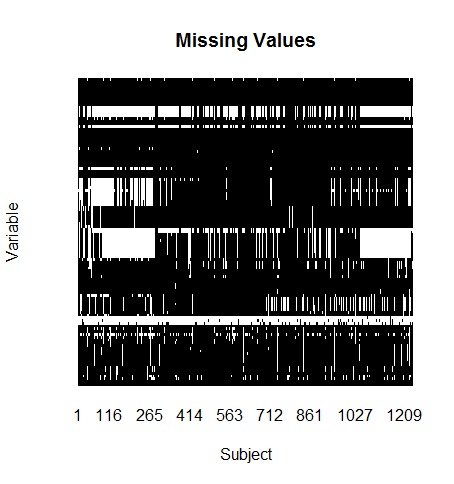
\includegraphics[width=0.5\textwidth]{missingvalues_plot.png}
  \caption{Visualization of missingness in the cancer dataset}
\label{fig:missingplot}

\end{figure}
\end{frame}



%%%%%%%%%%%

\begin{frame}{Plan For This Presentation}
Will put a graphic here of the flow of the paper
 
\end{frame}


\begin{comment}
 

\begin{frame}{Motivation}
\begin{itemize}
   \item This thesis is motivated by cancer survival data with moderate missingness
   \item We will build the theory for dealing with this situation
   \item And then apply it to a cancer data set
  \end{itemize}


\end{frame}

\begin{frame}{Abstract}
In this thesis, multiple imputation, survival analysis, and propensity score analysis are combined in 
order to answer questions about cancer data with moderate missingness. While each of these fields have 
been studied individually, there has been little work and analysis on using the three in trio.
Starting with an incomplete dataset, we aim to impute the missing data, run survival analysis on each
of the imputed datasets, and then do propensity score analysis to observe causal effects.
Along the way, many theoretical and analytical decisions are made. I explain why each decision is made, 
and offer ample evidence for the other choices such that the interested reader may implement the methods
if they so choose. I apply the methodology to a cancer survival dataset in a case study, but the methods 
used are general, and could be adapted for any type of data.
 
\end{frame}
\end{comment}


%\subsection{Missing data}
\begin{frame}{Plan For This Presentation}
  \begin{figure}[h!]
  \centering
    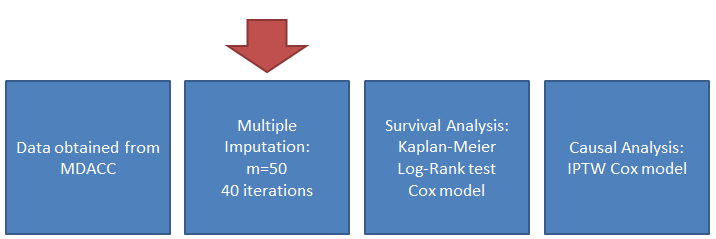
\includegraphics[width=0.9\textwidth]{mi_flow}
\label{fig:mi_flow}
\end{figure} 
\end{frame}

\begin{frame}{Missing data and Historical Approaches}
 \begin{itemize}
 \item Missing data happens when we intend to collect a piece of data but don't actually get it
 \item Historical approaches
 \begin{itemize}
  \item Complete Case (CC) analysis: Throw away any record that is not complete
  % list of downsides
 \item Available Case (AC) analysis: Use records so long as they are complete for the specific analysis in question
 %bad things here
 \item Single Imputation (SI): Fill in the missing value, deduct degrees of freedom to account for it
 \end{itemize}
 \end{itemize}
 
 \note{This can occur because when correlations are computed using different cases,
 the resulting patterns can be ones that are impossible to produce with complete data.}
\end{frame}

\begin{comment}
 
\begin{frame}{Imputation}
\begin{block}{Definition}
The English verb ``to impute'' comes from the Latin imputo, which means
to reckon, attribute, make account of, charge, ascribe. \cite{VanBuuren2012}
\end{block}
\begin{itemize}
 \item In the 1930's, Allan, Wishart, and Yates laid framework for missing data
 \begin{itemize}
  \item Idea: Fill in the missing value, deduct degrees of freedom to account for it
  \item Issue: Dogmatic, and variance can't be estimated correctly
 \end{itemize}

\end{itemize}
\end{frame}

\end{comment}

\begin{frame}{Multiple Imputation}
Throughout the 70's and 80's Donald Rubin worked to improve on single imputation
\begin{itemize}
 \item Instead of imputing one value, lets impute it $m\geq 2$ times
 \item Draw the values from the missing data's posterior distribution given the observed
 data and the process that generated the missing data
\end{itemize}
This idea is called Multiple Imputation (MI) and was formalized in 1987 \cite{Rubin1987}. It is the gold standard method
for missing data currently.

\note{MI are repitions drawn to simulate a Bayesian posterior distribution
of the missing values under a model}

\end{frame}


\begin{frame}{How does MI work?}
 \begin{figure}[h!]
  \centering
    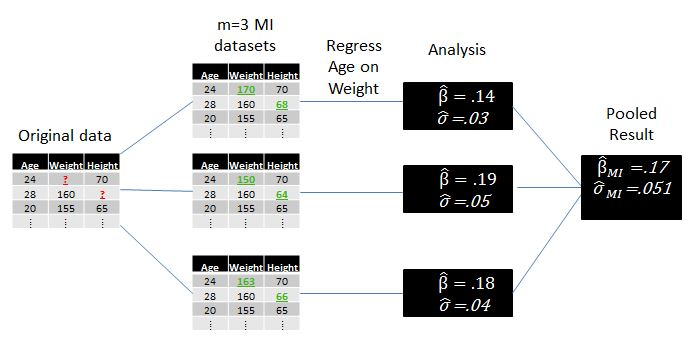
\includegraphics[width=0.8\textwidth]{mi_example_full.jpg}
  \caption{Visualization of MI data}
\label{fig:miexample}
\medskip
\small
Missingness is displayed by \textcolor{red}{?'s} and the imputed data is shown  as \textcolor{teal}{\#'s}.
We then regress age on weight, get the results from the individual datasets, and then pool them together.
\end{figure}
\note{We will go in to much more detail later in presentation}
\end{frame}

\begin{frame}{MI Theory}
 \begin{itemize}
  %\item Assume that the full data comes from $p(Y,X,R|\theta)$
  %\begin{itemize}
  % \item Y are the covariates with missingness
   %\item X is the fully observed covariates
   %\item R is the response missingness indicator
   %\item $\theta$ parameterizes this model
  %\end{itemize}
  \item Missing data model: $p(R|Y_{obs},Y_{mis},\psi)$
  \begin{itemize}
     \item R is the response missingness indicator
   \item $Y_{obs},Y_{mis}$ are observed and missings of Y (the set of covariates with missingness)
   \item $\psi$ parameterizes the missing data model
  \end{itemize}

 \end{itemize}

\end{frame}


\begin{frame}{Missing data Mechanisms}
%notation here?
\begin{itemize}

\item MCAR: Missing completely at random:  $$P(R=0|Y_{obs},Y_{mis},\psi)=P(R=0|\psi)$$
\begin{itemize}
\item The missingness in the data is not at all related to any of the data that we do or don't have
\end{itemize}
\item MAR: Missing at random: $$p(R=0|Y_{obs},Y_{mis},\psi)= p(R=0|Y_{obs},\psi)$$
\begin{itemize}
 \item The missingness we have is related to something in the data 
\end{itemize}
\item MNAR: Missing not at random: $$p(R=0|Y_{obs},Y_{mis},\psi)$$ does not simplify
\begin{itemize}
 \item  and the missingness depends on data that we have as well as have not collected
\end{itemize}
\end{itemize}
\note{
 If a lab technician slips and drops 5 vials of blood, the missingness caused by this would be MCAR
 If we collect the gender of the subject and we know that males tend to not give blood, we can attribute the missingness to the gender. In general, MAR models are ignorable.
 For example if a full moon causes the blood testing machine to break more often, but we don't have the moon phase as a variable.
}
\end{frame}

\begin{frame}{Missing data Example}

 \begin{figure}[h!]
  \centering
    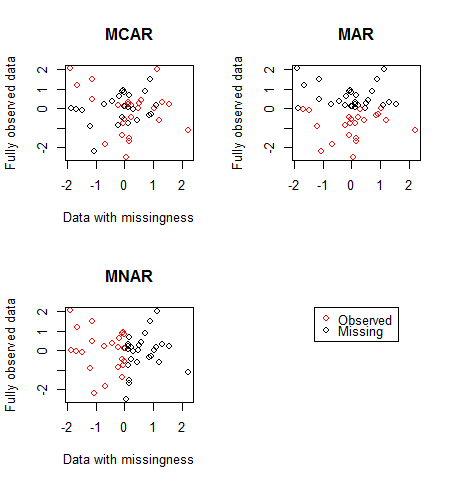
\includegraphics[width=0.63\textwidth]{md_mechanism}
  \caption{Visualization of MI data}
\label{fig:miviz}
\medskip
\small
Missingness is displayed by \textcolor{red}{?'s} and the imputed data is shown  as \textcolor{teal}{\#'s}.
We then regress age on weight, get the results from the individual datasets, and then pool them together.
\end{figure}
 
\end{frame}

\begin{frame}{Full Conditional Specification (FCS)}
 \begin{itemize}
  \item Assume MAR missing data mechanism %although MNAR with more 
  \item Missing data is imputed iteratively on a variable by variable basis
  \item Drawing from $p(Y,X,R|\theta)$ through the full conditionals $p(Y_j|X,Y_{-j},R,\theta_j)$
  \begin{itemize}
   \item X: Fully observed data
   \item $Y_{-j}$ is the missing components without column j
   \item $\theta$ parameterizes full data model
  \end{itemize}

  %\item Requires no distributional assumptions
  %\item Specify univariate models for each missing variable conditional on other variables
  \item Generalization of univariate imputation
  \item Idea: Specify k one dimensional models to impute on the missing data columns
 \end{itemize}

\end{frame}

%I'm going to want to type this up as an algorithm
\begin{frame}{FCS Algorithm- MICE}
  \begin{figure}[h!]
  \centering
    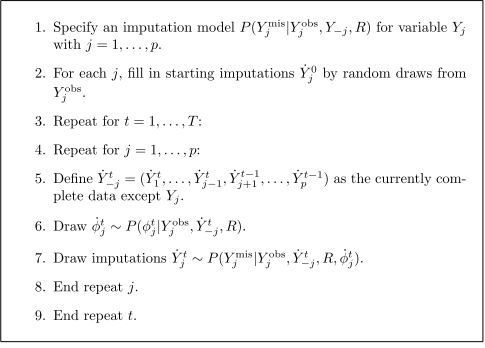
\includegraphics[width=0.6\textwidth]{fcs_algo}
  \caption{FCS imputation pseudocode, taken from \cite{VanBuuren2012}}
\label{fig:fcsexample}
\end{figure}
 \note{ Observe how the previous imputation Y_j^(t-1) only enters the current imputation
 through its relation with other variables, and not directly. This makes convergence very fast
}
\end{frame}

%moved this to intro 666
\begin{frame}{FCS Pros and Cons}
Pros
 \begin{itemize}
  \item Flexible
  \item Easy to specify models
  \item Handles mixed continuous categorical data
  \item Yeilds unbiased estimates with appropriate coverage
 \end{itemize}

 Cons
 \begin{itemize}
  \item No guarantee that full conditionals are compatible
  \item Takes time to set up
  \item Gets much harder as sample size increases to specify models
 \end{itemize}

\end{frame}

\begin{frame}{Imputation to the Cancer Data}

 \begin{itemize}
  \item MAR assumption seems reasonable
  %\item FCS over JM due to nature of data
  \item $m=50$ datasets
  \item 40 iterations
  %\item Check for convergence and validity
 \end{itemize}

\end{frame}

%issues were here


\begin{frame}{Convergence}
 
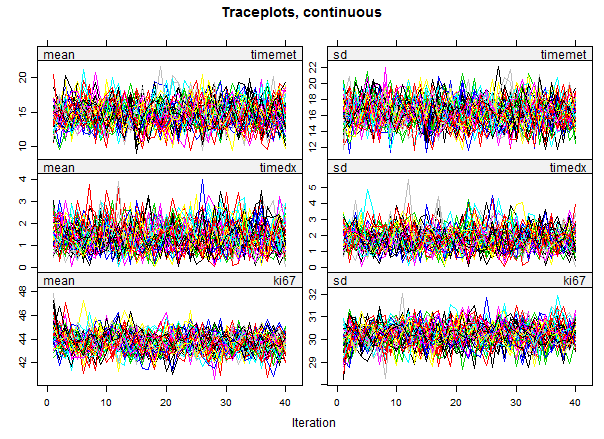
\includegraphics[width=.5\textwidth]{traceplots1}%
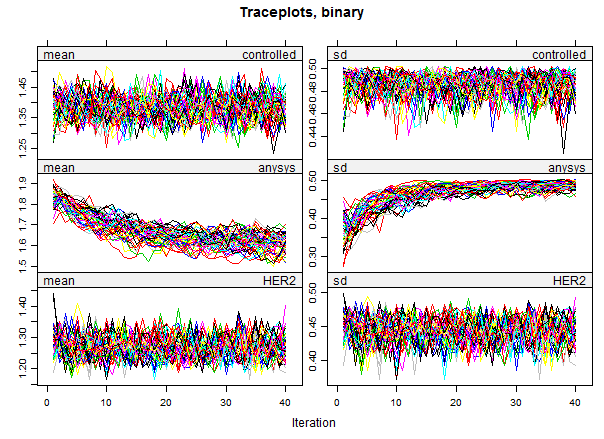
\includegraphics[width=.5\textwidth]{traceplots2} 

\note{On convergence, the different streams should be freely intermingled with one another,
without showing any definite trends. Convergence is diagnosed when the variance between different 
sequences is no larger than the variance within each individual sequence.
We do mean, because without it, we would have 50*missing num for each
var, and it would be very hard to read}

\end{frame}

\begin{frame}{Validity Checks}
%might want to pick better ones
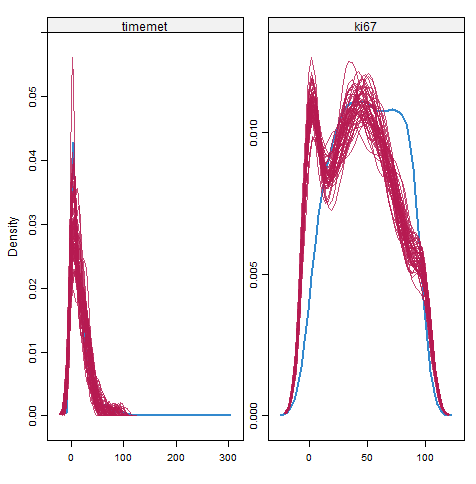
\includegraphics[width=.5\textwidth]{cont_densplot}%
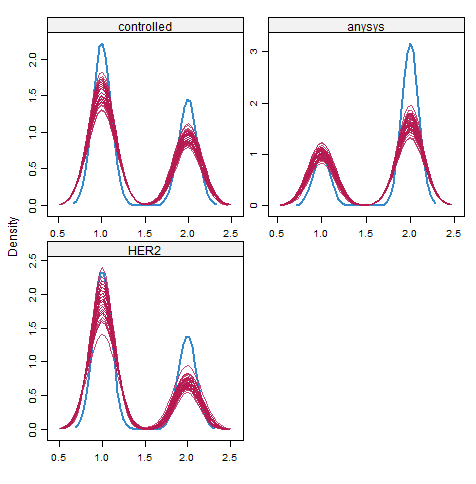
\includegraphics[width=.5\textwidth]{discrete_densplot} 
\end{frame}

\begin{frame}{MI data Breakdown}
\begin{table}[!ht]
\adjustbox{max height=\dimexpr\textheight-5.5cm\relax,
           max width=\textwidth}{
\centering
\begin{tabular}{|r|c|c|c|c|}
\hline
\multicolumn{1}{|l|}{}                            & \begin{tabular}[c]{@{}c@{}}Sys therapy \\ available case\end{tabular} & \begin{tabular}[c]{@{}c@{}}Sys therapy \\ MI\end{tabular} & \begin{tabular}[c]{@{}c@{}}No Sys therapy \\ available case\end{tabular} & \begin{tabular}[c]{@{}c@{}}No Sys therapy \\ MI\end{tabular} \\ \hline
\multicolumn{1}{|l|}{Age (mean,sd)}               & 51.4(10.8)                                                            & 51.2(10.9)                                                & 52.7(11.9)                                                               & 52.9(11.4)                                                   \\ \hline
\multicolumn{1}{|l|}{Breast Cancer subtype}       &                                                                       &                                                           &                                                                          &                                                              \\ \hline
HR+/HER2-                                         & 27\%                                                                  & 31\%                                                      & 28\%                                                                     & 33\%                                                         \\ \hline
HR+/HER2+                                         & 19\%                                                                  & 18\%                                                      & 12\%                                                                     & 13\%                                                         \\ \hline
HR-/HER2+                                         & 22\%                                                                  & 20\%                                                      & 15\%                                                                     & 12\%                                                         \\ \hline
Triple negative                                   & 32\%                                                                  & 32\%                                                      & 45\%                                                                     & 42\%                                                         \\ \hline
\multicolumn{1}{|l|}{Prior therapies for stage 4} & 1(0-3)                                                                & 2(0-4)                                                    & 2(0-4)                                                                   & 2(0-4)                                                       \\ \hline
\multicolumn{1}{|l|}{Single brain lesion}         & 25\%                                                                  & 23\%                                                      & 23\%                                                                     & 20\%                                                         \\ \hline
\multicolumn{1}{|l|}{Controlled extra-cranial}    & 40\%                                                                  & 40\%                                                      & 35\%                                                                     & 36\%                                                         \\ \hline
\multicolumn{1}{|l|}{ECOG 0-1}                    & 84\%                                                                  & 70\%                                                      & 53\%                                                                     & 40\%                                                         \\ \hline
\multicolumn{1}{|l|}{Local Therapy}               &                                                                       &                                                           &                                                                          &                                                              \\ \hline
Resection Alone                                   & 5\%                                                                   & 5\%                                                       & 9\%                                                                      & 7\%                                                          \\ \hline
SBRT alone                                        & 13\%                                                                  & 12\%                                                      & 9\%                                                                      & 8\%                                                          \\ \hline
WBRT                                              & 60\%                                                                  & 59\%                                                      & 52\%                                                                     & 53\%                                                         \\ \hline
Resection/SBRT+WBRT                               & 12\%                                                                  & 14\%                                                      & 10\%                                                                     & 8\%                                                          \\ \hline
no local therapy                                  & 10\%                                                                  & 10\%                                                      & 20\%                                                                     & 23\%                                                         \\ \hline
\end{tabular}
}
\caption{Characteristics of available case data versus MI data}
\label{table:chartab}
\end{table}
 
\end{frame}

\begin{frame}{Rubin's Rules}
 Let
 \begin{itemize}
  \item $\hat{Q}_i$ be the scientific estimand from the $i^{th}$ MI dataset
  \item $U_i$ be the variance-covariance matrix of the $i^{th}$ MI estimand
 \end{itemize}
Then
\begin{itemize}
 \item The MI estimate is given by
 $\bar{Q}=\frac{1}{m}\sum_{i=1}^{m}\hat{Q}_i$
 \item The MI ``within'' variance is given by
 $\bar{U}=\frac{1}{m}\sum_{i=1}^{m}U_i$
 \item the MI ``between'' variance is given by
 $B=\frac{1}{m-1}\sum_{i=1}^{m}(\hat{Q}_i - \bar{Q})(\hat{Q}_i - \bar{Q})'$ % matrix notation?
   \item Total variance given by \cite{Rubin1987}
  $$T=\bar{U}+B +\frac{B}{m}$$
\end{itemize}

\end{frame}

%I'm not sure where I want this to be 666
\begin{frame}{Inference with Rubin's Rules}
 \begin{itemize}
  \item Assume that with complete data, inference on the estimand
  Q would be based on the statement $(Q- \hat{Q})\sim N(0,U)$
  \begin{itemize}
   \item $\hat{Q}$ is the statistic estimating Q
   \item $U$ is the variance-covariance of $(Q-\hat{Q})$
  \end{itemize}
   \item Since true T is not known, then
  $$\frac{Q-\hat{Q}}{\sqrt{T}}\sim t_{\nu}$$
  \item $\nu$ is given by \cite{Barnard1999}
  $$\nu=\frac{\nu_{old}\nu_{obs}}{\nu_{old}+\nu_{obs}}$$
\item Where $\nu_{obs}=\frac{\nu_{com}+1}{\nu_{com}+3}\nu_{com}(1-\frac{B + B/m}{T})$
\item $\nu_{com}$ is the hypothetical complete sample degrees of freedom
\item $\nu_{old}=\frac{m-1}{(\frac{B + B/m}{T})^2}$ 
 \end{itemize}

 \note{Requires normality
if not normal, transform}
\end{frame}



%\subsection{Survival Analysis}
\begin{frame}{Survival Analysis}
\begin{block}{Survival Analysis}
Survival analysis is a field of statistics concerned with analyzing time to 
event data, often in the face of censoring or truncation.
\end{block}
Example:
\begin{itemize}
 \item The survival of patients after a liver transplant in a hospital
 \begin{itemize}
  \item Complications: study ending and no death, subject dies before study starts,
  subject moves away, exact death time is only known between two times
 \end{itemize}

\end{itemize}
\end{frame}

\begin{frame}{Kaplan-Meier Estimator}
\begin{itemize}
 \item The survival function $S(t)=P(T>t)=\int_{t}^{\infty}f(u)du$ is estimated by the 
 nonparametric Kaplan-Meier Estimator
 $$\hat{S}(t)=\prod_{t_i<t}\frac{n_i -d_i}{n_i}$$
\item $n_i$ is the number of subject in the risk set at time $t_i$
\item $d_i$ is the number of deaths at time $t_i$
\end{itemize}
 \begin{figure}[h!]
  \centering
    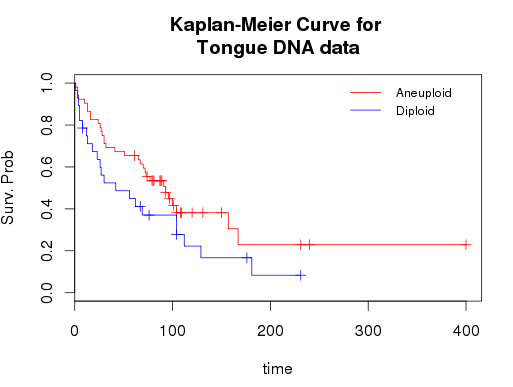
\includegraphics[width=0.45\textwidth]{km_example.png}
  \caption{A few different hazard function shapes, edited from wikipedia}
\label{fig:hazard}
\end{figure}
\note{
 risk set at time t; the set of individuals alive and uncensored just before time t.
We use death and survival because easy to say, but it really means event or not}
\end{frame}

\begin{frame}{Log rank test}
The log rank test compares two survival curves to see if from the same distribution

$$\frac{\sum_{j=1}^{J}(O_{1j}-E_{1j})}{\sqrt{\sum_{j=1}^{j}V_{j}}}\sim N(0,1)$$
\begin{itemize}
 \item $N_j=N_{1j}+N_{2j}$ is the number at risk at time j (composed from deaths in each group)
 \item $O_j=O_{1j}+O_{2j}$ is the observed number of deaths at time j (composed from the observed deaths in each group)
 \item $E_{1j}=\frac{O_jN_{1j}}{N_j}$
 \item $V_j=\frac{O_j(N_{1j}/N_j)(1-N_{1j}/N_j)(N_{j}-O_{j})}{N_j -1}$
 \end{itemize}
%\note[itemize]{ mention weights?
%}
\end{frame}


\begin{frame}{Hazard Function}
%might want to use the underbraces
%$\underbrace{h_{0}(t)}_{\textrm{time}}*\underbrace{exp(\sum_{k=1}^{p}\beta_{k}Z_{k})}_{\textrm{covariates}}$
\begin{itemize}
 \item Hazard is the instantaneous rate of event given that you have survived until time t, given 
 by $$h(t)=\lim_{\Delta t \rightarrow 0+}\frac{P[t\leq T<t+\Delta t|T\geq t]}{\Delta t}$$
\end{itemize}
 \begin{figure}[h!]
  \centering
    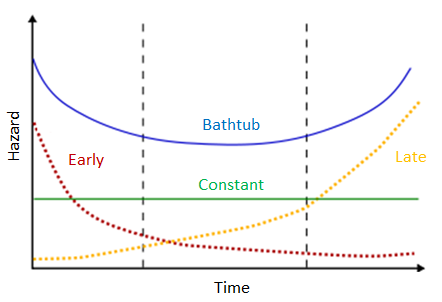
\includegraphics[width=0.65\textwidth]{hazard.png}
  \caption{A few different hazard function shapes, edited from wikipedia}
\label{fig:hazard}
\end{figure}
\end{frame}

\begin{frame}{Cox Regression}
\begin{itemize}
   \item Cox regression models hazard by 
   
   %$$h(t|Z)=h_{0}(t)\exp(\sum_{k=1}^{p}\beta_{k}Z_{k})$$
   $$h(t|Z)=\underbrace{h_{0}(t)}_{\textrm{time}}*\underbrace{exp(\sum_{k=1}^{p}\beta_{k}Z_{k})}_{\textrm{covariates}}$$

   \item Where $h_{0}(t)$ is the baseline hazard
   \item $Z_k$ is the $k^{th}$ covariate
   \item $\beta_k$'s are found by maximizing the partial likelihood function
\item The covariates act to multiply the hazard function.
\end{itemize}

\end{frame}


%\subsection{Causal Analysis}
\begin{frame}{Causal Analysis}
Suppose we have a new drug we want to test to see how efficacious it is.
 \begin{itemize}
  \item We would like to be able to say ``The drug leads to better health''
  \begin{itemize}
   \item But need an RCT to say this
   \begin{itemize}
    \item Randomization minimizes differences between groups at baseline
   \end{itemize}

   \item We only have observational data
   \item Thus differences could be attributed to the drug or confounding
   
   \begin{itemize}
    \item e.g. healthier people were much more likely to take the drug at baseline
   \end{itemize}

  \end{itemize}
Idea: Try to balance the covariates to reduce the effects of confounding
so the two groups seem identical at baseline
 \end{itemize}

\end{frame}

\begin{frame}{Counterfactual Model}
\begin{itemize}
 \item Suppose that for or every person, there are two potential outcomes
 \begin{itemize}
  \item $Y_i(0)$ - The outcome if they had taken the control, $Z=0$
  \item $Y_i(1)$ - The outcome if they had taken the treatment, $Z=1$
 \end{itemize}
\item Obviously, we only observe one. \textit{The fundamental problem of causal inference}
\item If we could observe both, then we could observe the causal effects for each person
\item Estimands of interest:
\begin{itemize}
 \item Average Treatment Effect (ATE) $E[Y_i(1)-Y_i(0)]$. The effect of moving entire population
 from treated to untreated
 \item Average treatment effect for the treated (ATT) $E[Y_i(1)-Y_i(0)|Z=1]$. The average treatment
 effect for those actually treated
\end{itemize}
\item In survival, the ATE is the difference in survival time
\end{itemize}
 
\end{frame}

\begin{frame}{Propensity scores}
\begin{block}{Definition}
The propensity score is the probability that the subject received the treatment given the subjects \textit{pretreatment}
covariates. It is computed using the patient's baseline (pretreatment) information \cite{Rosenbaum1983}
\end{block}
 \begin{itemize}
  \item Defined as  $e_i(x)=P(Z_i =1 |X_i)$
  \item Assume that the covariates play a role in how the subject chose treatment
  \item If we assume that $(Y(0),Y(1))\perp T|X \implies (Y(0),Y(1))\perp T|e(X)$
  \item Controlling for propensity score will make groups seem indistinguishable
  \item Thus, we may treat it as if it were an RCT
 \end{itemize}

\end{frame}

\begin{frame}{Common Propensity Score Methods}
\begin{itemize}
 \item Matching: Match treatment and controls on their propensity score, calculate ATE
 \item Stratification: Stratify on propensity score, weight and combine ATE in each strata
 \item Weighting: Weight each observation by the inverse of its propensity score, and then calculate ATE
\end{itemize}
\end{frame}

\begin{frame}{Propensity Score Issues}
 \begin{itemize}
  \item Unmeasured confounders
  \item Choice of pretreatment covariates in the propensity score model
  \item Different models and methods may lead to different conclusions
 \end{itemize}

\end{frame}


%\section{Methods}
%\subsection{Imputation}

%\begin{comment}
 
\begin{frame}{A path with many options}
 \begin{itemize}
  \item There are many different options to choose
  \item I explain my choices but discuss other options
  \item Goal: Be clear so other researchers can adapt my methodology to their problems
 \end{itemize}

\end{frame}

\begin{frame}{MI primer}
\begin{itemize}
 \item MI forms the base of this thesis
 \item There are lots of different ways to impute
 \item As long as we can impute valid imputations, we can analyze them
 \item Poor imputation leads to poor results (bias, variability, loss in power)
\end{itemize}
\end{frame}

\end{comment}

\begin{frame}{MI Notation}
 
 \begin{itemize}
\item $Y$ is our whole dataset. It will have $i$ rows and $j$ columns. Some of the covariates in the dataset will be completely observed, and others will have missingness.
\item $Y_j$ is a specific column of Y. $Y_j$ is composed as $Y_j=(Y_{j,obs},Y_{j,mis})$, where
	\begin{itemize}
	\item $Y_{j,obs}$ is the data we have observed for covariate j
	\item $Y_{j,mis}$ is the missing data covariate j
\end{itemize} 
\item $Y_{obs}$ is all of the data that we have observed
\item $Y_{mis}$ is all the data that we have not observed
\item R is a binary matrix the same size as $Y$ where a 1 indicates we observed the data, and 0 means it is missing
\item $\psi$ is a vector of parameters for the missing data model. 
\item The missing data model is given as $p(R|Y_{obs},Y_{mis},\psi)$
\item $\theta$ is a vector of the parameters for the full model of $Y$
\item $\phi_j$ is the unknown parameters of the imputation model 
\end{itemize}
\note{Missing data model relates Y to R}
\end{frame}

\begin{frame}{MI Concepts}
\begin{itemize}
 \item Ignorability
$$p(Y_{mis}|Y_{obs},R)= p(Y_{mis}|Y_{obs})$$
That is, we may ``ignore'' the R. The probability of the data being missing does not depend on how the data is missing. 
Equivalently, we may write this as
$$p(Y_{mis}|Y_{obs},R=1)= p(Y_{mis}|Y_{obs},R=0)$$
\item Non ignorability: $$p(Y_{mis}|Y_{obs},R=1)\neq p(Y_{mis}|Y_{obs},R=0)$$
So we must take into account the missing data structure for imputation.


\end{itemize}

\note{Being ignorable makes it justified to model our missing data from our observed data, without needing to worry about how it was missing.
The opposite of ignorable data is called non-ignorable data, in this case.
We often times see ignorable missing data in practice,
although one should certainly check the sensibility of ignorability, as some instances will certainly be non-ignorable, 
for example censored data, or when we know that the missing data is systematically different than the observed. 
If we have strongly nonignorable data, we should either try one of two things.

The first is to expand the data (collect something else similar to the covariate with missingness) so that it becomes ignorable and 

the second is to formulate two imputation models, one for the observed and one for the missing.

}

\end{frame}

\begin{frame}{Missing data Mechanisms}
Now, we may discuss the three main types of missing data mechanisms. 
\begin{itemize}

\item MCAR: Missing completely at random:  $$P(R=0|Y_{obs},Y_{mis},\psi)=P(R=0|\psi)$$
\begin{itemize}
\item The missingness in the data is not at all related to any of the data that we do or don't have
\end{itemize}
\item MAR: Missing at random: $$p(R=0|Y_{obs},Y_{mis},\psi)= p(R=0|Y_{obs},\psi)$$
\begin{itemize}
 \item The missingness we have is related to something in the data 
\end{itemize}
\item MNAR: Missing not at random: $$p(R=0|Y_{obs},Y_{mis},\psi)$$ does not simplify
\begin{itemize}
 \item  and the missingness depends on data that we have as well as have not collected
\end{itemize}


\end{itemize}
\note{
 If a lab technician slips and drops 5 vials of blood, the missingness caused by this would be MCAR
 If we collect the gender of the subject and we know that males tend to not give blood, we can attribute the missingness to the gender. In general, MAR models are ignorable.
 For example if a full moon causes the blood testing machine to break more often, but we don't have the moon phase as a variable.
}
 
\end{frame}

%JM wa here

\begin{frame}{Full Conditional Specification (FCS)}
 \begin{itemize}
  \item Assume MAR missing data mechanism %although MNAR with more 
  \item Missing data is imputed iteratively on a variable by variable basis
  \item Requires no distributional assumptions
  \item Idea: Specify k one dimensional models to impute on the missing data columns
 \end{itemize}

\end{frame}

\begin{frame}{FCS Algorithm}
  \begin{figure}[h!]
  \centering
    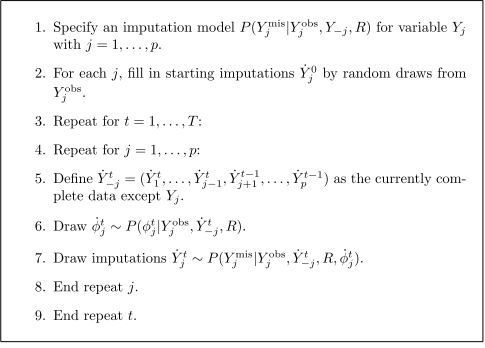
\includegraphics[width=0.6\textwidth]{fcs_algo}
 % \caption{Normal JM imputation pseudocode}
\label{fig:fcsexample}
\end{figure}
 \note{ Observe how the previous imputation Y_j^(t-1) only enters the current imputation
 through its relation with other variables, and not directly. This makes convergence very fast
}
\end{frame}

\begin{frame}{FCS Pros and Cons}
Pros
 \begin{itemize}
  \item Flexible
  \item Easy to specify models
  \item Handles mixed continuous categorical
 \end{itemize}

 Cons
 \begin{itemize}
  \item No guarantee that full conditionals are compatible
  \item Slow
  \item Gets much harder as sample size increases to specify models
 \end{itemize}

\end{frame}

\begin{comment}
 
\begin{frame}{Decision}
 \begin{itemize}
  \item Both are not as good as having complete data
  \item Cancer and survival data present challenges for JM
  \item FCS offers us the most ease and flexibility
 \end{itemize}
\end{frame}

\end{comment}

\begin{frame}{Setting Up The Model}
\begin{itemize}
 \item Specify the models
 \item Specify the predictors for each model
 \item Determine number of iterations and datasets to impute
 \begin{itemize}
  \item This is a topic of hot debate
  \item Old literature suggested 5 imputations, 5 iterations, but more now
 \end{itemize}

\end{itemize}

\note{Many disagreements, but all say at least 5}
\end{frame}

\begin{frame}{Checking The Imputations}
 Convergence
 \begin{itemize}
  \item Chains should be freely intermingled with no pattern
  \item Convergence when variance between chains is no larger than variance within each chain
  \item Formal tests like Gelman/Rubin $\hat{R}$ proposed to check convergence
 \end{itemize}
Validation
\begin{itemize}
 \item ``Does the data look like it could have come from real data had it not been missing''?
 \begin{itemize}
  \item Requires intimate knowledge of the data
 \end{itemize}
\item Graphical checks
\begin{itemize}
 \item Density plots
 \item Conditional scatter plots
 \item Box and whisker
 \item etc.
\end{itemize}

\end{itemize}
\end{frame}

\begin{frame}{Pooling}
 \begin{itemize}
  \item We now have $m$ imputed datasets
  \item Run the analysis on each of the $m$ complete datasets
  \item But we want one analysis, not $m$
 \end{itemize}

\end{frame}

\begin{frame}{Rubin's Rules}
 Let
 \begin{itemize}
  \item $\hat{Q}_i$ be the scientific estimand from the $i^{th}$ MI dataset
  \item $U_i$ be the variance-covariance matrix of the $i^{th}$ MI estimand
 \end{itemize}
Then
\begin{itemize}
 \item The MI estimate is given by
 $\bar{Q}=\frac{1}{m}\sum_{i=1}^{m}\hat{Q}_i$
 \item The MI ``within'' variance is given by
 $\bar{U}=\frac{1}{m}\sum_{i=1}^{m}U_i$
 \item the MI ``between'' variance is given by
 $B=\frac{1}{m-1}\sum_{i=1}^{m}(\hat{Q}_i - \bar{Q})(\hat{Q}_i - \bar{Q})'$ % matrix notation?
   \item Total variance given by \cite{Rubin1987}
  $$T=\bar{U}+B +\frac{B}{m}$$
\end{itemize}

\end{frame}

%tidy this up
\begin{frame}{Inference with Rubin's Rules}
 \begin{itemize}
  \item Assume that with complete data, inference on the estimand
  Q would be based on the statement $(Q- \hat{Q})\sim N(0,U)$
  \begin{itemize}
   \item $\hat{Q}$ is the statistic estimating Q
   \item $U$ is the variance-covariance of $(Q-\hat{Q})$
  \end{itemize}
   \item Since true T is not known, then
  $$\frac{Q-\hat{Q}}{\sqrt{T}}\sim t_{\nu}$$
  \item $\nu$ is given by \cite{Barnard1999}
  $$\nu=\frac{\nu_{old}\nu_{obs}}{\nu_{old}+\nu_{obs}}$$
\item Where $\nu_{obs}=\frac{\nu_{com}+1}{\nu_{com}+3}\nu_{com}(1-\frac{B + B/m}{T})$
\item $\nu_{com}$ is the hypothetical complete sample degrees of freedom
\item $\nu_{old}=\frac{m-1}{(\frac{B + B/m}{T})^2}$ 
 \end{itemize}

 \note{Requires normality
if not normal, transform}
\end{frame}


%stack method was here
%\subsection{Survival}
%\begin{frame}{Kaplan-Meier in the MI Setting}
 \begin{itemize}
  \item Clearly define the population, groups, and events of interest
  \item Ensure that we have noninformative censoring
  \item Issue: Kaplan-Meier is not normally distributed
  \begin{itemize}
   \item Solution: Complimentary log log transformation, pool \cite{Marshall2009}
  \end{itemize}
  \item Issue: Imputations leave one KM curve much shorter than the rest
  \begin{itemize}
   \item Solution 1: Truncate all curves at the lowest time
   \item Solution 2: Extend the curves out to the longest time
   \item Solution 3: Use the stacked method
  \end{itemize}
\item Algorithm: Pool the complimentary log log of the Kaplan-Meier curve, get estimates,
back transform
 \end{itemize}

\end{frame}

%I want to make this better
\begin{frame}{Median Survival Time}
 \begin{itemize}
  \item Want a measure of central tendency
  \begin{itemize}
   \item Survival distributions often skewed, so mean is poor choice
  \end{itemize}
  \item Median: smallest time such that $\hat{S}(t)\leq .5$
\item Algorithm: Take MI Kaplan-Meier curve, observe first time it goes below 50\%
\item Confidence interval at median: Take the median of the upper and lower confidence bands
 \end{itemize}

\end{frame}

\begin{frame}{Log Rank Test}
 \begin{itemize}
  \item Idea: Combine log rank tests from each MI dataset
  \begin{itemize}
  \item Problem: Wastes information and is unstable \cite{Marshall2009}
  \item Idea: Calculate log rank from the MI Kaplan-Meier curve
  \item Problem: Risk set and deaths no longer meaningful
  \end{itemize}

  \item Solution: Under no tied times, the score test on
  Cox Regression on a treatment is equivalent to the
log rank test
\begin{itemize}
 \item And very similar under tied times
\end{itemize}
\item Idea: Derive log rank test from Cox model
\begin{itemize}
 \item Pooling LRT and Score test is unstable \cite{Marshall2009}
 \item Wald test is asymptotically equivalent
\end{itemize}
 \item Final Solution: Run the Wald test on Cox model as an approximation

 \end{itemize}

\end{frame}

\begin{frame}{Cox Model in the MI Setting}
\begin{itemize}
 \item Goal: To get a ``baseline'' Cox model, then add treatment variables
 \item Need to check for proportional hazards assumption
 \begin{itemize}
  \item Problem:  MI Cox model doesn't have residuals
  \item Solution: Check assumptions (Schoenfeld residuals) on stacked dataset or each MI dataset individually
 \end{itemize}
\item Cox model is normally distributed, use Rubin's Rules to pool
\item Add treatment covariates, rerun models, pool
\end{itemize}

 
\end{frame}


%\subsection{Causal Analysis}
%\begin{frame}{Propensity Score}
\begin{itemize}
 \item How to use the propensity score
 \begin{itemize}
  \item Matching, weighting, covariate adjustment, stratification
 \end{itemize}
\item Generating the propensity score
\begin{itemize}
 \item Logistic regression, Probit regression, CART, etc.
\end{itemize}
\item Verifying balance
\end{itemize} 
\end{frame}

\begin{frame}{Propensity Score in MI Setting}
\begin{itemize}
 \item Mitra and Reiter propose two methods \cite{Mitra2012}
 \item Within: Work with propensity score on each of the $m$ MI datasets
 \item Across: Average propensity scores across the $m$ datasets and then analyze
 \item Which to use: Dependent on your data
\end{itemize}

 
\end{frame}


%\section{Application}
%\subsection{Breast Brain Mets Example}

%\begin{frame}{Data Explanation}
\begin{itemize}
 \item 1514 MD Anderson patients who had brain mets from breast cancer between 19XX and 20XX
 \item 1242 usable cases
 \item 90 covariates
 \begin{itemize}
  \item Missingness from 0 to 65\%
 \end{itemize}

\end{itemize}
\begin{table}[!ht]
\centering
\begin{tabular}{|c|c|}
\hline
Type                                                                            & Example                                                                       \\ \hline
Subject data                                                                    & Age range, race, date of birth                                                \\ \hline
Breast Cancer data                                                                     & TNM staging, type, receptor status                                            \\ \hline
\begin{tabular}[c]{@{}c@{}}Pre brain mets\\ data\end{tabular}                   & Treatment types                                                               \\ \hline
\begin{tabular}[c]{@{}c@{}}Post brain mets\\ clinical observations\end{tabular} & Seizures, headache, nausea                                                    \\ \hline
\begin{tabular}[c]{@{}c@{}}Post brain mets\\ data\end{tabular}                  & \begin{tabular}[c]{@{}c@{}}Treatment type, \\ type of brain mets\end{tabular} \\ \hline
Survival data                                                                   & Survival time after brain mets, censoring indicator                           \\ \hline
\end{tabular}
\caption{Data Categories and Examples}
\label{table:cats}
\end{table}

\end{frame}

\begin{frame}{Questions of interest}
Want to explore...
\begin{itemize}
 \item Chemotherapeutic drugs: Capecitabine vs other chemotherapeutic agents
 \item HER2 directed therapies (Lapatinib, Trastuzumab) in HER2+ subjects
 \item Note: treatment not determined at time of diagnosis, need to landmark (2 months)
 
 \note{Human epidermal growth factor receptor 2 (HER2) overexpression drives the biology of 20
 pct of breast cancers, and predicts a poor prognosis for patients.}
\end{itemize}

 
\end{frame}


\begin{frame}{Important Covariates}
 \begin{table}[ !ht]
\centering
\adjustbox{max height=\dimexpr\textheight-5.5cm\relax,
           max width=\textwidth}{
\begin{tabular}{|c|c|c|}
\hline
Name        & \begin{tabular}[c]{@{}c@{}}Percent \\ Missing\end{tabular} & Meaning                                                                                                                                             \\ \hline
hrher2      & 5                                                        & \begin{tabular}[c]{@{}c@{}}Categorical variable: The hormonal receptor and \\ HER2 receptor status of the subject\end{tabular}                      \\ \hline
agebrainmet & 0                                                          & Indicator: Age greater or less than 60 at time of brain mets                                                                                        \\ \hline
timedx      & 1                                                         & \begin{tabular}[c]{@{}c@{}}Indicator: Time (years) from breast cancer diagnosis to brain\\ mets diagnosis greater or less than 6 years\end{tabular} \\ \hline
site5       & 1                                                        & Indicator: First metastasis was to brain                                                                                                            \\ \hline
race2       & 0                                                          & Categorical: White, Black, Hispanic, other                                                                                                          \\ \hline
priorn      & 0                                                          & \begin{tabular}[c]{@{}c@{}}Indicator: Number of prior treatments in metastatic setting \\ before brain mets\end{tabular}                            \\ \hline
braintype   & 4                                                        & Categorical: Single, multiple, Leptomeningeal disease                                                                                               \\ \hline
controlled  & 12                                                        & Indicator: Extracranial progression of brain mets                                                                                                   \\ \hline
capeothno   & 18                                                        & \begin{tabular}[c]{@{}c@{}}Indicator: Capecitabine, other, or no chemotherapeutic\\ treatment. Treatment variable 1\end{tabular}                     \\ \hline
lapatrasno  & 18                                                        & \begin{tabular}[c]{@{}c@{}}Indicator: Lapatinib, Trastuzumab, or no HER2 treatment.\\ Treatment variable 2\end{tabular}                             \\ \hline
os          & 0                                                          & Overall survival (months)                                                                                                                           \\ \hline
dead        & 0                                                          & Indicator: death indicator                                                                                                                          \\ \hline
her2        & 10                                                        & Indicator: HER2 receptor status                                                                                                                     \\ \hline
\end{tabular}
}
\caption{Table of important covariates to be used in the analysis}
\label{table:importantvars}

\end{table}
\end{frame}

\begin{frame}{Visualization of Missingness}
 \begin{figure}[h!]
  \centering
    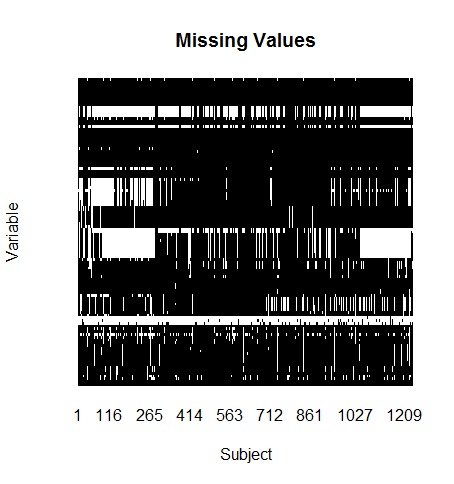
\includegraphics[width=0.8\textwidth]{missingvalues_plot.png}
  \caption{Visualization of missingness in the cancer dataset}
\label{fig:missingplot}

\end{figure}
\end{frame}

\begin{frame}{Imputation}
 \begin{itemize}
  \item MAR assumption seems reasonable
  \item FCS over JM due to nature of data
  \item Need to set up models and predictors
  \item Check for convergence and validity
 \end{itemize}

\end{frame}

\begin{frame}{Setting up the model}
Issues
\begin{itemize}
 \item Many categorical variables 
 \item Collinearity between predictors
 \item Variables with poor influx/outflux \cite{VanBuuren2012}
 \item How many iterations and imputations to draw?
\end{itemize}

 
\end{frame}


\begin{frame}{Convergence}
 
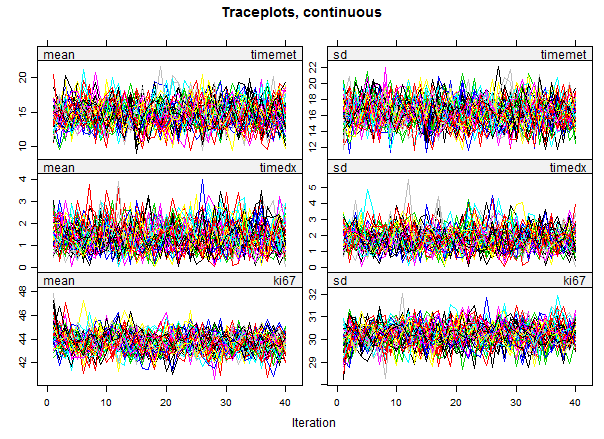
\includegraphics[width=.5\textwidth]{traceplots1}%
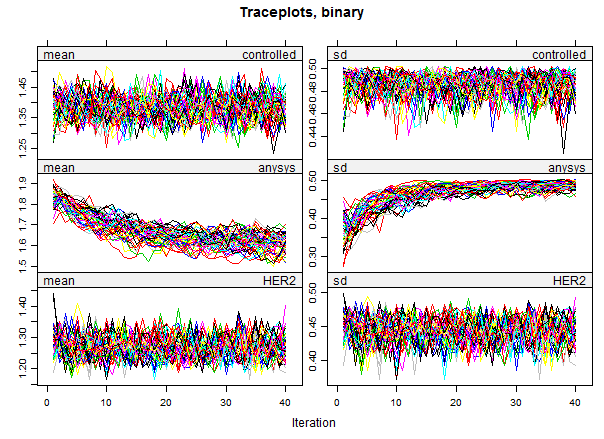
\includegraphics[width=.5\textwidth]{traceplots2} 

\note{On convergence, the different streams should be freely intermingled with one another,
without showing any definite trends. Convergence is diagnosed when the variance between different 
sequences is no larger than the variance within each individual sequence.
We do mean, because without it, we would have 50*missing num for each
var, and it would be very hard to read}

\end{frame}

\begin{frame}{Validity}
 \begin{itemize}
  \item Lots of tools for continuous imputations
  \item Not many for categorical
  \begin{itemize}
   \item Solution: look at tables to verify validity
  \end{itemize}

 \end{itemize}

\end{frame}

\begin{frame}{Validity Checks}
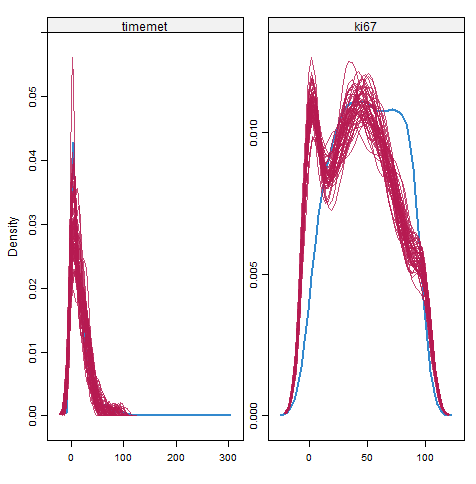
\includegraphics[width=.5\textwidth]{cont_densplot}%
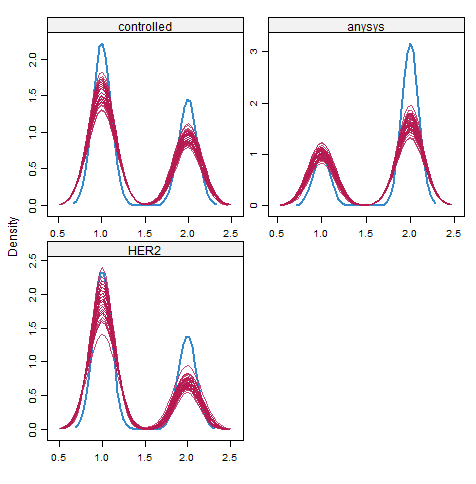
\includegraphics[width=.5\textwidth]{discrete_densplot} 
\end{frame}

\begin{frame}{Validity Checks}
 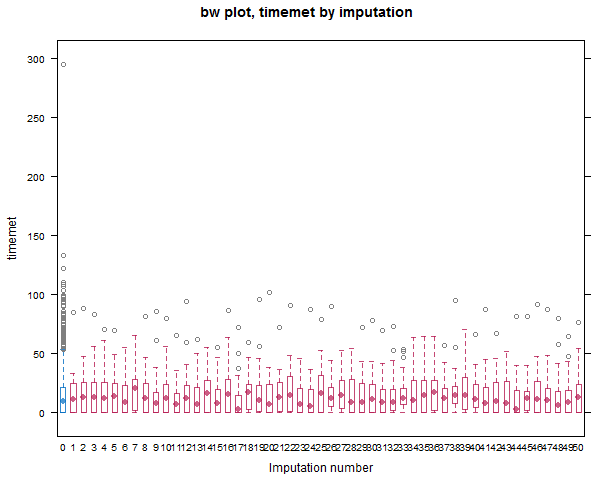
\includegraphics[width=.5\textwidth]{bw_timemet}%
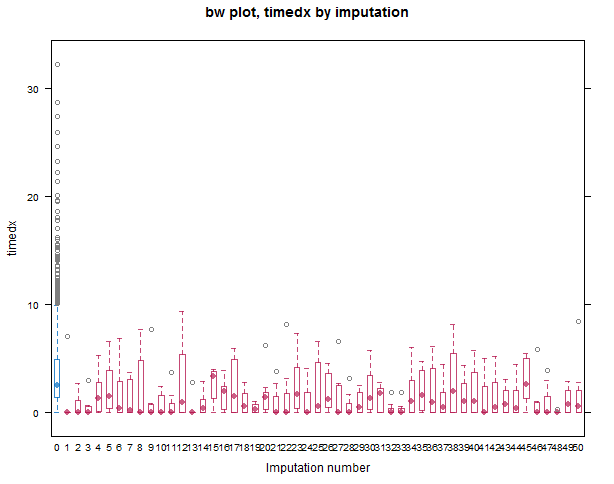
\includegraphics[width=.5\textwidth]{bw_timedx} 
\end{frame}

\begin{frame}{Tabluar Checks}
 \begin{figure}[h!]
  \centering
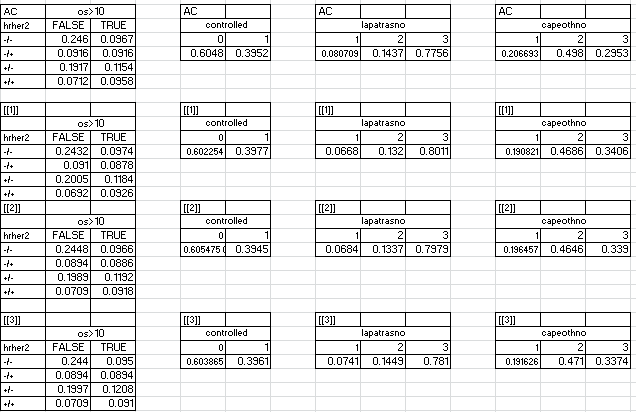
\includegraphics[width=.8\textwidth]{tabchecks} 
  \caption{Selected tabluar checks}
\label{fig:tabcheck}
\end{figure}

\end{frame}

\begin{frame}{MI data Breakdown}
\begin{table}[!ht]
\adjustbox{max height=\dimexpr\textheight-5.5cm\relax,
           max width=\textwidth}{
\centering
\begin{tabular}{|r|c|c|c|c|}
\hline
\multicolumn{1}{|l|}{}                            & \begin{tabular}[c]{@{}c@{}}Sys therapy \\ available case\end{tabular} & \begin{tabular}[c]{@{}c@{}}Sys therapy \\ MI\end{tabular} & \begin{tabular}[c]{@{}c@{}}No Sys therapy \\ available case\end{tabular} & \begin{tabular}[c]{@{}c@{}}No Sys therapy \\ MI\end{tabular} \\ \hline
\multicolumn{1}{|l|}{Age (mean,sd)}               & 51.4(10.8)                                                            & 51.2(10.9)                                                & 52.7(11.9)                                                               & 52.9(11.4)                                                   \\ \hline
\multicolumn{1}{|l|}{Breast Cancer subtype}       &                                                                       &                                                           &                                                                          &                                                              \\ \hline
HR+/HER2-                                         & 27\%                                                                  & 31\%                                                      & 28\%                                                                     & 33\%                                                         \\ \hline
HR+/HER2+                                         & 19\%                                                                  & 18\%                                                      & 12\%                                                                     & 13\%                                                         \\ \hline
HR-/HER2+                                         & 22\%                                                                  & 20\%                                                      & 15\%                                                                     & 12\%                                                         \\ \hline
Triple negative                                   & 32\%                                                                  & 32\%                                                      & 45\%                                                                     & 42\%                                                         \\ \hline
\multicolumn{1}{|l|}{Prior therapies for stage 4} & 1(0-3)                                                                & 2(0-4)                                                    & 2(0-4)                                                                   & 2(0-4)                                                       \\ \hline
\multicolumn{1}{|l|}{Single brain lesion}         & 25\%                                                                  & 23\%                                                      & 23\%                                                                     & 20\%                                                         \\ \hline
\multicolumn{1}{|l|}{Controlled extra-cranial}    & 40\%                                                                  & 40\%                                                      & 35\%                                                                     & 36\%                                                         \\ \hline
\multicolumn{1}{|l|}{ECOG 0-1}                    & 84\%                                                                  & 70\%                                                      & 53\%                                                                     & 40\%                                                         \\ \hline
\multicolumn{1}{|l|}{Local Therapy}               &                                                                       &                                                           &                                                                          &                                                              \\ \hline
Resection Alone                                   & 5\%                                                                   & 5\%                                                       & 9\%                                                                      & 7\%                                                          \\ \hline
SBRT alone                                        & 13\%                                                                  & 12\%                                                      & 9\%                                                                      & 8\%                                                          \\ \hline
WBRT                                              & 60\%                                                                  & 59\%                                                      & 52\%                                                                     & 53\%                                                         \\ \hline
Resection/SBRT+WBRT                               & 12\%                                                                  & 14\%                                                      & 10\%                                                                     & 8\%                                                          \\ \hline
no local therapy                                  & 10\%                                                                  & 10\%                                                      & 20\%                                                                     & 23\%                                                         \\ \hline
\end{tabular}
}
\caption{Characteristics of available case data versus MI data}
\label{table:chartab}
\end{table}
 
\end{frame}

\begin{frame}{Kaplan-Meier in MI}
 \begin{itemize}
  \item Non-informative censoring reasonable
  \item Pooled by Rubin's Rules on Complimentary log-log
 \end{itemize}
 \begin{figure}[h!]
  \centering
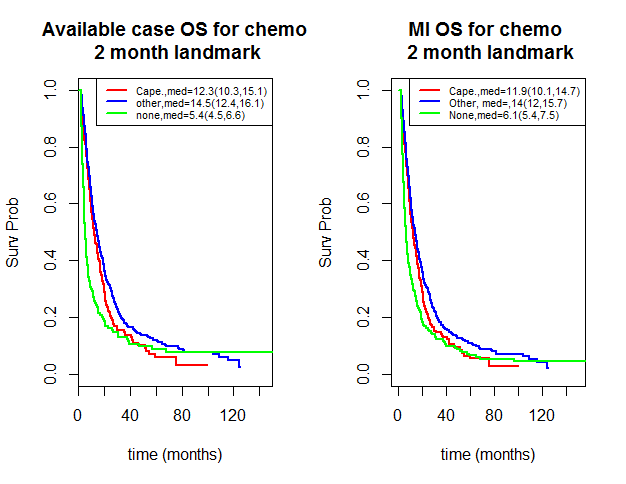
\includegraphics[width=.75\textwidth]{cape_km}
\end{figure}
\end{frame}




\begin{frame}{Kaplan-Meier in MI}
 \begin{figure}[h!]
  \centering
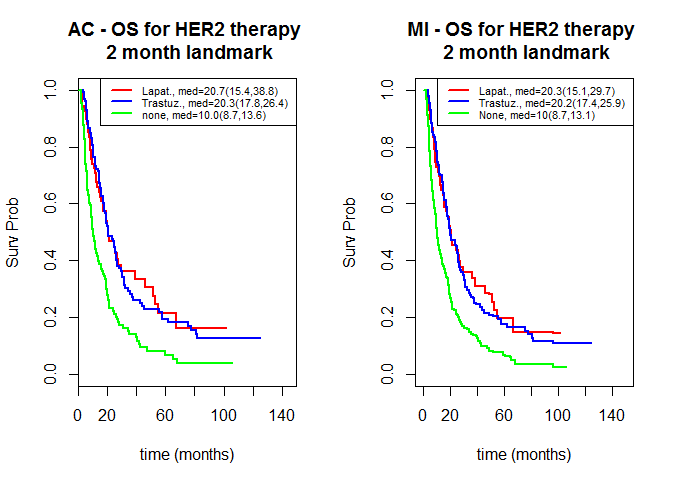
\includegraphics[width=.8\textwidth]{lapat_km}
\end{figure}
 
\end{frame}

\begin{frame}{Log Rank Test}
\begin{table}[]
\centering
\begin{tabular}{|l|c|c|}
\hline
                & \multicolumn{2}{c|}{Chemo}                         \\ \hline
                & \multicolumn{1}{l|}{AC} & \multicolumn{1}{l|}{MI} \\ \hline
cape/other/none & \textless.0001          & \textless.0001          \\ \hline
cape/other      & 0.0321                  & 0.033                   \\ \hline
cape/none       & 0.00039                 & .0016                   \\ \hline
other/none      & \textless.0001          & \textless.0001          \\ \hline
\end{tabular}
\end{table}
%
\begin{table}[]
\centering
\begin{tabular}{|l|c|c|}
\hline
                   & \multicolumn{2}{c|}{HER2}                         \\ \hline
                   & \multicolumn{1}{l|}{AC} & \multicolumn{1}{l|}{MI} \\ \hline
Lapat/Traztuz/none & \textless.0001          & \textless.0001          \\ \hline
Lapat/Trastuz      & .87                     & .81                     \\ \hline
Lapat/none         & .00017                  & .00018                  \\ \hline
Trastuz/none       & \textless.0001          & \textless.0001          \\ \hline
\end{tabular}
\end{table}
\end{frame}

\begin{comment}
 
\begin{frame}{Cox Model in MI}
\begin{itemize}
 \item Get good baseline model
 \item Need to check proportional hazards
 \item Add treatment variables
\end{itemize}
\end{frame}

\end{comment}

\begin{frame}{Schoenfeld Residual Splines}
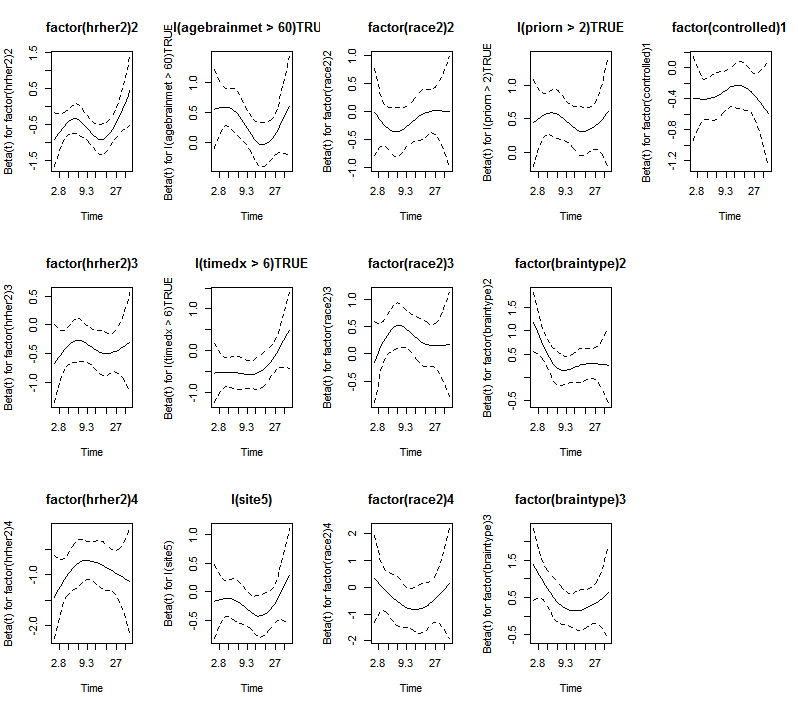
\includegraphics[width=.5\textwidth]{ac_schoenfeld}%
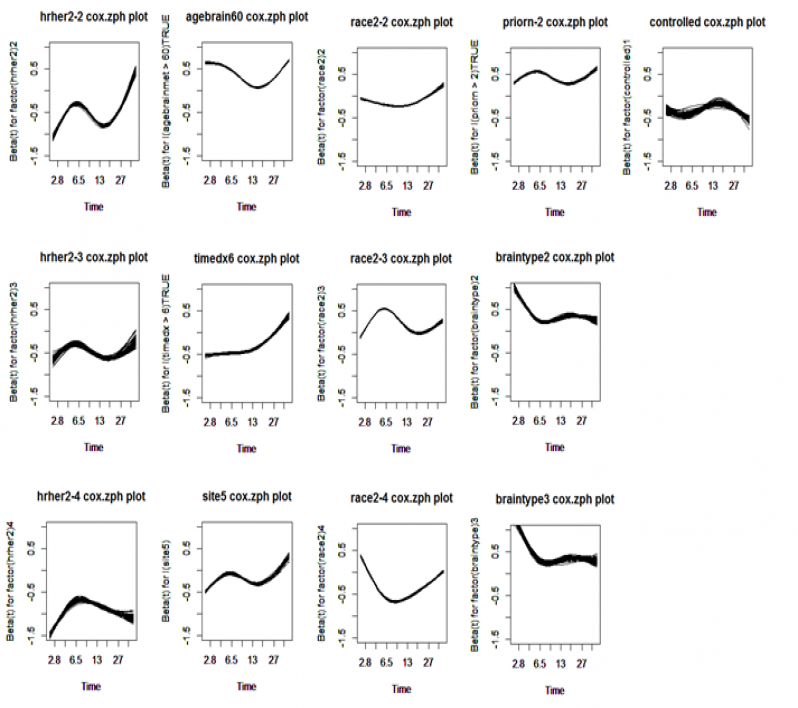
\includegraphics[width=.5\textwidth]{mi_schoenfeld} 
\end{frame}

\begin{frame}{Base model}
 \begin{table}[]
\centering
\adjustbox{max height=\dimexpr\textheight-5.5cm\relax,
           max width=\textwidth}{
\begin{tabular}{|c|c|c|c|c|c|c|c|c|}
\hline
                                                       &                                  &      & \begin{tabular}[c]{@{}c@{}}AC \\ n= 845\end{tabular} &                 &  &      & MI                                                 &                                                            \\ \hline
Variable                                               & Contrast                         & HR   & \begin{tabular}[c]{@{}c@{}}95\% \\ CI\end{tabular}   & pvalue          &  & HR   & \begin{tabular}[c]{@{}c@{}}95\% \\ CI\end{tabular} & \begin{tabular}[c]{@{}c@{}}pvalue\\  (t test)\end{tabular} \\ \hline
HR/HER2                                                & -/+ vs. -/-                      & 0.57 & (0.46,0.71)                                          & \textless0.0001 &  & 0.59 & (0.48,0.72)                                        & \textless0.0001                                            \\ \hline
                                                       & +/- vs. -/-                      & 0.66 & (0.54,0.81)                                          & \textless0.0001 &  & 0.63 & (0.52,0.76)                                        & \textless0.0001                                            \\ \hline
                                                       & +/+ vs. -/-                      & 0.4  & (0.31,0.50)                                          & \textless0.0001 &  & 0.4  & (0.32,0.50)                                        & \textless0.0001                                            \\ \hline
Age                                                    & \textgreater 60 vs. \textless 60 & 1.37 & (1.13,1.65)                                          & 0.0011          &  & 1.45 & (1.22,1.72)                                        & \textless0.0001                                            \\ \hline
Dx to BM                                               & \textgreater 6 vs. \textless 6   & 0.66 & (0.54,0.82)                                          & 0.00013         &  & 0.71 & (0.59,0.86)                                        & 0.0002                                                     \\ \hline
First DM                                               & Brain vs. Oth                    & 0.8  & (0.66,0.97)                                          & 0.026           &  & 0.83 & (0.70,0.99)                                        & 0.02                                                       \\ \hline
Race                                                   & Hisp. Vs. White                  & 0.85 & (0.68,1.07)                                          & 0.17            &  & 0.88 & (0.71,1.08)                                        & 0.11                                                       \\ \hline
                                                       & Black vs. White                  & 1.31 & (1.06,1.63)                                          & 0.014           &  & 1.25 & (1.02,1.52)                                        & 0.015                                                      \\ \hline
                                                       & Other vs. White                  & 0.65 & (0.40,1.04)                                          & 0.075           &  & 0.7  & (0.45,1.07)                                        & 0.05                                                       \\ \hline
\begin{tabular}[c]{@{}c@{}}\# prior \\ Rx\end{tabular} & \textgreater2 vs. 0-2            & 1.58 & (1.31,1.91)                                          & \textless0.0001 &  & 1.53 & (1.29,1.82)                                        & \textless0.0001                                            \\ \hline
BM type                                                & Mult. Vs. Single                 & 1.45 & (1.20,1.76)                                          & \textless0.0001 &  & 1.48 & (1.24,1.76)                                        & \textless0.0001                                            \\ \hline
                                                       & LMD vs. Single                   & 1.6  & (1.21,2.13)                                          & 0.001           &  & 1.58 & (1.25,2.00)                                        & \textless0.0001                                            \\ \hline
Sys. Cont.                                             & Yes vs. No                       & 0.71 & (0.61,0.83)                                          & \textless0.0001 &  & 0.73 & (0.63,0.85)                                        & \textless0.0001                                            \\ \hline
\end{tabular}
}
\caption{AC and MI baseline Cox model}
\label{fig:acmicox}
\end{table}

\end{frame}

\begin{frame}{MI Cox Model, Chemo}
\begin{table}[]
\centering
\adjustbox{max height=.9\dimexpr\textheight-5.5cm\relax,
           max width=\textwidth}{
\begin{tabular}{|l|l|c|c|c|c|c|c|c|}
\hline
                               &                                  &  &  \begin{tabular}[c]{@{}c@{}}AC\\ n= 745\end{tabular}& \multicolumn{1}{l|}{} & \multicolumn{1}{l|}{} & \multicolumn{1}{l|}{} & MI          & \multicolumn{1}{l|}{}                                       \\ \hline
\multicolumn{1}{|c|}{Variable} & \multicolumn{1}{c|}{Contrast}    & HR                                                  & 95\% CI               & p-value               & \multicolumn{1}{l|}{} & HR                    & 95\% CI     & \begin{tabular}[c]{@{}c@{}}p-value \\ (t test)\end{tabular} \\ \hline
HR/HER2                        & -/+ vs. -/-                      & 0.62                                                & (0.49,0.79)           & \textless .0001       &                       & 0.63                  & (0.51,0.77) & \textless .0001                                             \\ \hline
                               & +/- vs. -/-                      & 0.65                                                & (0.53,0.81)           & 0.00011               &                       & 0.64                  & (0.53,0.78) & \textless .0001                                             \\ \hline
                               & +/+ vs. -/-                      & 0.41                                                & (0.31,0.53)           & \textless .0001       &                       & 0.42                  & (0.34,0.53) & \textless .0001                                             \\ \hline
Age                            & \textgreater 60 vs. \textless 60 & 1.34                                                & (1.10,1.64)           & 0.0041                &                       & 1.44                  & (1.21,1.72) & \textless .0001                                             \\ \hline
Dx to BM                       & \textgreater 6 vs. \textless 6   & 0.72                                                & (0.58,0.90)           & 0.0032                &                       & 0.71                  & (0.58,0.86) & 0.00039                                                     \\ \hline
First DM                       & Brain vs. Oth                    & 0.77                                                & (0.63,0.95)           & 0.014                 &                       & 0.81                  & (0.68,0.96) & 0.016                                                       \\ \hline
Race                           & Hisp. Vs. White                  & 0.77                                                & (0.61,0.98)           & 0.034                 &                       & 0.86                  & (0.69,1.06) & 0.15                                                        \\ \hline
                               & Black vs. White                  & 1.29                                                & (1.02,1.63)           & 0.032                 &                       & 1.23                  & (1.01,1.51) & 0.043                                                       \\ \hline
                               & Other vs. White                  & 0.76                                                & (0.47,1.25)           & 0.28                  &                       & 0.7                   & (0.45,1.08) & 0.11                                                        \\ \hline
\# prior Rx                    & \textgreater2 vs. 0-2            & 1.61                                                & (1.32,1.98)           & \textless .0001       &                       & 1.53                  & (1.28,1.82) & \textless .0001                                             \\ \hline
BM type                        & Mult. Vs. Single                 & 1.46                                                & (1.20,1.78)           & 0.00017               &                       & 1.51                  & (1.27,1.81) & \textless .0001                                             \\ \hline
                               & LMD vs. Single                   & 1.45                                                & (1.04,2.03)           & 0.029                 &                       & 1.41                  & (1.11,1.80) & 0.0049                                                      \\ \hline
Sys. Cont.                     & Yes vs. No                       & 0.57                                                & (0.48,0.68)           & \textless .0001       &                       & 0.69                  & (0.59,0.80) & \textless .0001                                             \\ \hline
Chemo                          & Cape. vs. none                   & 0.69                                                & (0.53,0.89)           & 0.0046                &                       & 0.75                  & (0.60,0.95) & 0.018                                                       \\ \hline
                               & other vs. none                   & 0.52                                                & (0.42,0.65)           & \textless .0001       &                       & 0.58                  & (0.47,0.71) & \textless .0001                                             \\ \hline
\end{tabular}
}
\caption{AC and MI Cox model with Chemo Treatment}
\label{acmi_cox_chemo}
\end{table} 
\end{frame}

\begin{frame}{AC and MI Cox Model with HER2 Treatment}
\begin{table}[]
\centering
\adjustbox{max height=\dimexpr\textheight-5.5cm\relax,
           max width=\textwidth}{
\begin{tabular}{|l|l|c|c|c|c|c|c|c|}
\hline
                               &                                  & \multicolumn{1}{l|}{} & \begin{tabular}[c]{@{}c@{}}AC\\ n=292\end{tabular} & \multicolumn{1}{l|}{} & \multicolumn{1}{l|}{} &      & \begin{tabular}[c]{@{}c@{}}MI\\ n between 391\\ and 415\end{tabular} & \multicolumn{1}{l|}{}                                       \\ \hline
\multicolumn{1}{|c|}{Variable} & \multicolumn{1}{c|}{Contrast}    & HR                    & 95\% CI                                            & p-value               &                       & HR   & 95\% CI                                                              & \begin{tabular}[c]{@{}c@{}}p-value \\ (t test)\end{tabular} \\ \hline
HR/HER2                        & +/+ vs. -/+                      & 0.65                  & (0.49,0.87)                                        & 0.0036                &                       & 0.66 & (0.51,0.85)                                                          & 0.0015                                                      \\ \hline
Age                            & \textgreater 60 vs. \textless 60 & 1.38                  & (0.95,2.01)                                        & 0.092                 &                       & 1.58 & (1.15,2.18)                                                          & 0.0054                                                      \\ \hline
Dx to BM                       & \textgreater 6 vs. \textless 6   & 0.64                  & (0.43,0.97)                                        & 0.033                 &                       & 0.69 & (0.49,0.99)                                                          & 0.041                                                       \\ \hline
First DM                       & Brain vs. Oth                    & 0.84                  & (0.58,1.20)                                        & 0.34                  &                       & 0.86 & (0.62,1.17)                                                          & 0.34                                                        \\ \hline
Race                           & Hisp. Vs. White                  & 0.69                  & (0.46,1.02)                                        & 0.064                 &                       & 0.76 & (0.53,1.09)                                                          & 0.14                                                        \\ \hline
                               & Black vs. White                  & 1.41                  & (0.94,2.11)                                        & 0.1                   &                       & 1.43 & (1.00,2.04)                                                          & 0.047                                                       \\ \hline
                               & Other vs. White                  & 0.7                   & (0.32,1.53)                                        & 0.38                  &                       & 0.83 & (0.46,1.52)                                                          & 0.55                                                        \\ \hline
\# prior Rx                    & \textgreater2 vs. 0-2            & 1.88                  & (1.34,2.63)                                        & 0.00028               &                       & 1.71 & (1.28,2.28)                                                          & 0.00028                                                     \\ \hline
BM type                        & Mult. Vs. Single                 & 1.3                   & (0.92,1.86)                                        & 0.14                  &                       & 1.25 & (0.91,1.70)                                                          & 0.16                                                        \\ \hline
                               & LMD vs. Single                   & 2.15                  & (1.20,3.88)                                        & 0.011                 &                       & 1.77 & (1.10,2.83)                                                          & 0.018                                                       \\ \hline
Sys. Cont.                     & Yes vs. No                       & 0.73                  & (0.55,0.97)                                        & 0.029                 &                       & 0.78 & (0.60,1.01)                                                          & 0.063                                                       \\ \hline
HER2 therapy                   & Lapat vs. none                   & 0.47                  & (0.32,0.69)                                        & 0.00015               &                       & 0.52 & (0.37,0.75)                                                          & 0.00036                                                     \\ \hline
                               & Trastuz vs. none                 & 0.45                  & (0.33,0.61)                                        & \textless.0001        &                       & 0.51 & (0.38,0.68)                                                          & \textless.0001                                              \\ \hline
\end{tabular}
}
\caption{AC and MI Cox model with HER2 Treatment}

\end{table}
\end{frame}

\begin{frame}{Causal Analysis}
\begin{itemize}
 \item Need to get propensity score from \textit{pretreatment} covariates
 \item Check the balance and standardized bias
 \item Run IPTW analysis on each dataset
 \item Use Mitra and Reiter's within method to get each MI dataset ATE \cite{Mitra2012}
 \item Pool via Rubin's Rules
\end{itemize}
\end{frame}

 
%causal issues were here


\begin{frame}{IPTW Weighting in MI Setting}
\begin{itemize}
 \item Set the propensity score model - GBM
 \begin{itemize}
  \item Confounding factors: stage, race, IDC, breast cancer surgery, HR/HER2 status,
  breast cancer radiation, first met site, number of prior treatments, ECOG score,
  localized brain mets treatment, age at brain met, type of brain mets, brain met controlled
 \end{itemize}

 \item Weight observations by propensity score
 \item Check to ensure balance achieved -KS and standardized bias
 \item Run IPTW weighted Cox regression on treatment
 \item Pool results via Rubin's rules
 %\item Double robustness: Include pretreatment variables in model?
\end{itemize} 
\end{frame}


\begin{frame}{Implementation}
 \begin{itemize}
  \item A few of the balance diagnostics
  \item results
 \end{itemize}

\end{frame}

\begin{frame}{Results of IPTW}
 \begin{table}[]
\centering
\adjustbox{max height=\dimexpr\textheight-5.5cm\relax,
           max width=\textwidth}{
\begin{tabular}{|l|l|l|l|l|l|l|l|}
\hline
               & AC-Unweighted &  & AC-Weighted &  & MI unweighted &  & MI Weighted \\ \hline
Cape. vs none  & 0.396         &  & 0.655       &  & 0.484         &  & 0.702       \\ \hline
Other vs none  & 0.336         &  & 0.567       &  & 0.413         &  & 0.593       \\ \hline
Cape vs. other & 1.179         &  & 1.156       &  & 1.173         &  & 1.183      \\ \hline
\end{tabular}
}
\caption{Chemotherapeutic ATE with IPTW weights, AC and MI}

\end{table}

\begin{table}[]
\centering
\begin{tabular}{|l|c|c|c|c|c|c|c|c|c|c|c|}
\hline
                   & \multicolumn{2}{c|}{AC Unweighted}                              & \multicolumn{1}{l|}{} & \multicolumn{2}{c|}{AC IPTW}                                    & \multicolumn{1}{l|}{} & \multicolumn{2}{c|}{MI no weight}                              & \multicolumn{1}{l|}{} & \multicolumn{2}{c|}{MI IPTW}                                    \\ \hline
                   & HR                         & 95\% CI                            &                       & HR                         & 95\% CI                            &                       & HR                         & 95\% CI                           &                       & HR                         & 95\% CI                            \\ \hline
Lapat. vs none     & 0.467                      & (0.355,0.616)                      &                       & 0.571                      & (0.381,0.855)                      &                       & 0.474                      & (0.362,0.622)                     &                       & 0.485                      & (0.304,0.775)                      \\ \hline
Trastuz. vs none   & 0.488                      & (0.398,0.597)                      &                       & 0.566                      & (0.421,0.759)                      &                       & 0.506                      & (0.417,0.614)                     &                       & 0.480                      & (0.313,0.735)                      \\ \hline
Lapat. vs Trastuz. & \multicolumn{1}{l|}{0.958} & \multicolumn{1}{l|}{(0.693,1.324)} & \multicolumn{1}{l|}{} & \multicolumn{1}{l|}{1.009} & \multicolumn{1}{l|}{(0.680,1.496)} & \multicolumn{1}{l|}{} & \multicolumn{1}{l|}{0.927} & \multicolumn{1}{l|}{(0.673,1.28)} & \multicolumn{1}{l|}{} & \multicolumn{1}{l|}{1.011} & \multicolumn{1}{l|}{(0.763,1.338)} \\ \hline
\end{tabular}
\caption{HER2 directed ATE with IPTW weights, AC and MI}
\label{tab:lapatonly}
\end{table}
 
\end{frame}



\begin{frame}{Critiques}
 \begin{itemize}
  \item MI doubters and method critiques
  \item Assumptions in the survival section
  \item Propensity score in general and model choices
 \end{itemize}

\end{frame}

\begin{frame}{Further research}

\begin{itemize}
 \item Differing imputation methods
 \item Competing risks
 \item AFT models
 \item Differing propensity score methods
 \item Estimating counterfactuals as an MI problem in MI setting
 
\end{itemize}

 
\end{frame}

\begin{frame}{Any Questions?}
\begin{itemize}
 \item Any questions?
\end{itemize}
\end{frame}


\appendix
\section{Extras}

\begin{frame}{Supplemental Slides}
 
 \begin{itemize}
  \item Discuss in depth topics should time allow
 \end{itemize}

\end{frame}

\begin{frame}{Propensity Score Issues}
 \begin{itemize}
  \item Unmeasured confounders
  \item Choice of pretreatment covariates in the propensity score model
  \item Different models and methods may lead to different conclusions
 \end{itemize}

\end{frame}

\begin{frame}{Joint Modelling (JM)}
 \begin{itemize}
  \item Assume ignorable MAR  missing data mechanism
  \item Missing data imputed by sampling from a user specified distribution
  \item A lot of theory developed for Normal, not much else
  \begin{itemize}
   \item Normal imputation has been shown to perform well, even under non normality \cite{Demirtas2008}
  \end{itemize}
\item Idea: pull imputations by missing data row pattern
 \end{itemize}

\end{frame}

\begin{frame}{JM pseudocode}
 \begin{figure}[h!]
  \centering
    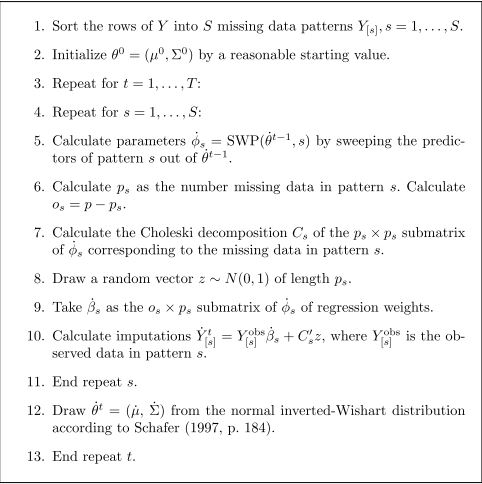
\includegraphics[width=0.6\textwidth]{jm_algo}
 % \caption{Normal JM imputation pseudocode}
\label{fig:jmexample}
\end{figure}
%do I want to include the amelia algo?
\end{frame}

\begin{frame}{JM Pros and Cons}
Pros
 \begin{itemize}
  \item Fast
  \item Easy to derive posteriors with common distributions
 \end{itemize}

 Cons
 \begin{itemize}
  \item Inflexible
  \item Limited to known distributions
  \item How to deal with mixed categorical and continuous missing data
 \item Poor with derived variables
 \item Can give impossible combinations
 \end{itemize}

\end{frame}



\begin{frame}{Inference with Rubin's Rules}
 \begin{itemize}
  \item Assume that with complete data, inference on the estimand
  Q would be based on the statement $(Q- \hat{Q})\sim N(0,U)$
  \begin{itemize}
   \item $\hat{Q}$ is the statistic estimating Q
   \item $U$ is the variance-covariance of $(Q-\hat{Q})$
  \end{itemize}
   \item Since true T is not known, then
  $$\frac{Q-\hat{Q}}{\sqrt{T}}\sim t_{\nu}$$
  \item $\nu$ is given by \cite{Barnard1999}
  $$\nu=\frac{\nu_{old}\nu_{obs}}{\nu_{old}+\nu_{obs}}$$
\item Where $\nu_{obs}=\frac{\nu_{com}+1}{\nu_{com}+3}\nu_{com}(1-\frac{B + B/m}{T})$
\item $\nu_{com}$ is the hypothetical complete sample degrees of freedom
\item $\nu_{old}=\frac{m-1}{(\frac{B + B/m}{T})^2}$ 
 \end{itemize}

 \note{Requires normality
if not normal, transform}
\end{frame}

\begin{frame}{The Stack Method}
 \begin{itemize}
  \item Rubin's Rules work well, but not always
  \begin{itemize}
   \item Ex: partitioning the MI data on an imputed variable
   \item Taking the average is not a good idea
  \end{itemize}
    \item Solution: Stack the MI datasets on top of each other to get one huge dataset
    \begin{itemize}
     \item Will get unbiased results
     \item But sample size is falsely inflated, thus cannot trust variance
    \end{itemize}
 \end{itemize}
 \begin{figure}[h!]
  \centering
    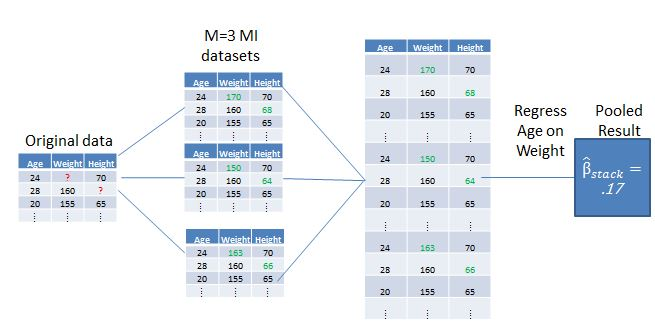
\includegraphics[width=0.6\textwidth]{stacked}
 % \caption{Normal JM imputation pseudocode}
\label{fig:stacked}
\end{figure}
\end{frame}

\begin{frame}{KM issues in the MI setting}
\begin{itemize}
\item Issue: Kaplan-Meier is not normally distributed
  \begin{itemize}
   \item Solution: Complimentary log log transformation, pool \cite{Marshall2009}
  \end{itemize}
  \item Issue: Imputations leave one KM curve much shorter than the rest
  \begin{itemize}
   \item Solution 1: Truncate all curves at the lowest time
   \item Solution 2: Extend the curves out to the longest time
   \item Solution 3: Use the stacked method
  \end{itemize}

\end{itemize}
\end{frame}

\begin{frame}{Log Rank Issues in MI setting}
\begin{itemize}
  \item Idea: Combine log rank tests from each MI dataset
  \begin{itemize}
  \item Problem: Wastes information and is unstable \cite{Marshall2009}
  \item Idea: Calculate log rank from the MI Kaplan-Meier curve
  \item Problem: Risk set and deaths no longer meaningful
  \end{itemize}
\end{itemize}
\end{frame}

\begin{frame}{Setting up the model- Issues}
\begin{itemize}
 \item Many categorical variables 
 \item Collinearity between predictors
 \item Variables with poor influx/outflux \cite{VanBuuren2012}
 \item How many iterations and imputations to draw?
\end{itemize}

\end{frame}


\begin{frame}{Validity Checks}
 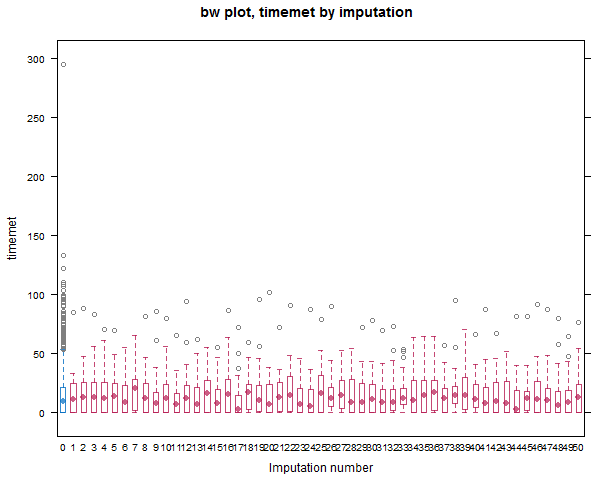
\includegraphics[width=.5\textwidth]{bw_timemet}%
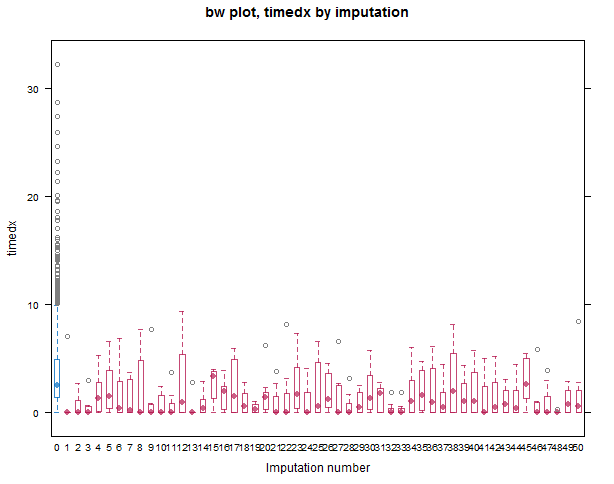
\includegraphics[width=.5\textwidth]{bw_timedx} 
\end{frame}

\begin{frame}{Tabluar Checks}
 \begin{figure}[h!]
  \centering
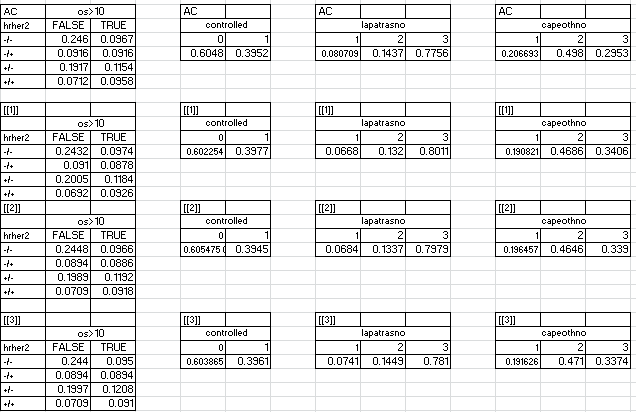
\includegraphics[width=.8\textwidth]{tabchecks} 
  \caption{Selected tabluar checks}
\label{fig:tabcheck}
\end{figure}

\end{frame}


\begin{frame}{Issues with Propensity Score in our Setting}
\begin{itemize}
 \item Problem: Theory was developed for binary treatments, we have ternary
 \begin{itemize}
  \item Solution: Run each treatment as binary, then compare groups
 \end{itemize}
\item Propensity score model specification
\begin{itemize}
 \item Solution: Boosting, subject to KS statistic minimization
\end{itemize}
\end{itemize}
 
\end{frame}

%put boosting algo here if I have time

\begin{comment}
 

% You can reveal the parts of a slide one at a time
% with the \pause command:
\begin{frame}{Second Slide Title}
  \begin{itemize}
  \item {
    First item.
    \pause % The slide will pause after showing the first item
  }
  \item {   
    Second item.
  }
  % You can also specify when the content should appear
  % by using <n->:
  \item<3-> {
    Third item.
  }
  \item<4-> {
    Fourth item.
  }
  % or you can use the \uncover command to reveal general
  % content (not just \items):
  \item<5-> {
    Fifth item. \uncover<6->{Extra text in the fifth item.}
  }
  \end{itemize}
\end{frame}

\section{Second Main Section}

\subsection{Another Subsection}

\begin{frame}{Blocks}
\begin{block}{Block Title}
You can also highlight sections of your presentation in a block, with it's own title
\end{block}
\begin{theorem}
There are separate environments for theorems, examples, definitions and proofs.
\end{theorem}
\begin{example}
Here is an example of an example block.
\end{example}
\end{frame}

% Placing a * after \section means it will not show in the
% outline or table of contents.
\section*{Summary}

\begin{frame}{Summary}
  \begin{itemize}
  \item
    The \alert{first main message} of your talk in one or two lines.
  \item
    The \alert{second main message} of your talk in one or two lines.
  \item
    Perhaps a \alert{third message}, but not more than that.
  \end{itemize}
  
  \begin{itemize}
  \item
    Outlook
    \begin{itemize}
    \item
      Something you haven't solved.
    \item
      Something else you haven't solved.
    \end{itemize}
  \end{itemize}
\end{frame}



% All of the following is optional and typically not needed. 
\appendix
\section<presentation>*{\appendixname}
\subsection<presentation>*{For Further Reading}
\begin{comment}
 

\begin{frame}[allowframebreaks]
  \frametitle<presentation>{For Further Reading}
    
  \begin{thebibliography}{10}
    
  \beamertemplatebookbibitems
  % Start with overview books.

  \bibitem{Author1990}
    A.~Author.
    \newblock {\em Handbook of Everything}.
    \newblock Some Press, 1990.
 
    
  \beamertemplatearticlebibitems
  % Followed by interesting articles. Keep the list short. 

  \bibitem{Someone2000}
    S.~Someone.
    \newblock On this and that.
    \newblock {\em Journal of This and That}, 2(1):50--100,
    2000.
  \end{thebibliography}
\end{frame}
\end{comment}

\begin{frame}[allowframebreaks]
        \frametitle{References}
        \bibliographystyle{ieeetr}
	\bibliography{Research}
\end{frame}
\end{document}


